\documentclass[a4paper, 12pt, oneside]{tesisutec}

% Location of the graphics files (set up for graphics to be in PDF format)
\graphicspath{images/}

% Include any extra LaTeX packages required
\usepackage[square, numbers, comma, sort&compress]{natbib}
\usepackage{verbatim}  %
\usepackage[spanish]{babel}
\selectlanguage{spanish}

\makeatletter
% Reinsert missing \algbackskip
\def\algbackskip{\hskip-\ALG@thistlm}
\makeatother

\usepackage{float}
\usepackage[spanish,onelanguage,ruled,vlined]{algorithm2e}

\hypersetup{urlcolor=blue, colorlinks=true}


%
\usepackage{notoccite}  
\usepackage{hyperref} 

% For Spanish
\usepackage[utf8]{inputenc}

%% ============================================================================
\begin{document}

\degree{Maestro en Ciencia de Datos e Inteligencia Artificial}
\title{NEXUSCARE: SOLUCIÓN DE AUDITORÍA AUTOMATIZADA DE LIQUIDACIONES MÉDICAS BASADA EN INTELIGENCIA ARTIFICIAL}

\author{Roberto Carlos Hurtado Crisostomo \orcid{0009-0000-3650-7792} \\ Javier Linares Gonzales \orcid{0009-0000-3650-7792}}
\supervisor{Renzo Otoniel Osso Sanchez \orcid{0009-0000-4577-1384}}

\date{2026}

\maketitle
\thispagestyle{empty} 
\setcounter{page}{1}  

\setstretch{1.5}
\thispagestyle{empty}   
\addtocounter{page}{1}  


\fancypagestyle{plain}{
  \fancyhf{} % limpia cabecera y pie
}

\renewcommand{\contentsname}{\Large \bfseries TABLA DE CONTENIDO}




\tableofcontents
\newpage
\renewcommand{\listtablename}{\Large \bfseries ÍNDICE DE TABLAS}
\listoftables
\thispagestyle{empty}
\newpage
\renewcommand{\listfigurename}{\Large \bfseries ÍNDICE DE FIGURAS}
\listoffigures
\thispagestyle{empty}
\newpage
\addtocontents{toc}{\vspace{1.5em}}


\chapter*{\center \Large \vspace{-4.5cm} ÍNDICE DE ANEXOS}
\listofannexes
\thispagestyle{empty}
%% ============================================================================
\pagestyle{fancy}
\chapter*{\center \Large \vspace{-4.5cm} RESUMEN}
\addcontentsline{toc}{section}{RESUMEN}
\markboth{RESUMEN}{RESUMEN} 
\thispagestyle{empty}
\spacing{1.25}\noindent
La auditoría de liquidaciones médicas hospitalarias en Perú es un proceso predominantemente manual consumiendo entre 30 y 45 minutos por caso. Un lote típico de 101 liquidaciones requiere 75.8 horas de trabajo por auditor médico especializado, gran parte dedicada a casos rutinarios de bajo riesgo. Este trabajo presenta a NexusCare, un agente de auditoría clínica que combina un motor determinístico de reglas contractuales (Fase 1) con modelos de lenguaje de gran escala (Fase 2) para clasificar cada liquidación según su riesgo clínico-económico y priorizar la revisión especializada.

La selección de modelos utilizó un \textit{benchmark} de cinco LLM (Claude Sonnet 4, Claude Opus 4.6, GPT-5.4, Gemini 2.5 Pro y MedGemma 27B) sobre 101 liquidaciones, totalizando 505 evaluaciones. Sonnet 4 mostró la mayor capacidad de discriminación ($\sigma$ = 20.1), mientras otros modelos presentaron sesgos de sobrepenalización. Se adoptó una estrategia escalonada: Sonnet evalúa el 100 \% de los casos y escala el 33 \% a Opus, reduciendo el costo en 57 \% frente al uso exclusivo de Opus.

El \textit{pipeline} integrado alcanzó 65.3 \% de recomendaciones \textit{fast-track}, con 66 casos de bajo riesgo validables en aproximadamente un minuto, un costo de API de USD 12.00 y 38.9 minutos de procesamiento. La recalibración de umbrales (+41.6 pp), los \textit{prompts} anti-sesgo (+6.0 pp) y el prefiltrado contractual (-7.0 pp) explican el desempeño. La reducción estimada del tiempo total de auditoría oscila entre 57 \% y 72 \%, superando la meta de 40 \%. La validación operativa en producción queda como siguiente paso.

\chapter*{\center \Large \vspace{-4.5cm} ABSTRACT}
\addcontentsline{toc}{section}{ABSTRACT}
\markboth{ABSTRACT}{ABSTRACT} 
\thispagestyle{empty}
\begin{center}
\Large \vspace{-1.5cm} \textbf{NEXUSCARE: AI-BASED AUTOMATED AUDIT SOLUTION FOR MEDICAL CLAIMS}
\end{center}

\spacing{1.25}\noindent
The auditing of hospital medical claims in Peru is a predominantly manual process, consuming between 30 and 45 minutes per case. A typical batch of 101 claims requires 75.8 hours of work per specialized medical auditor, much of it devoted to routine, low-risk cases. This work presents NexusCare, a clinical audit agent that combines a deterministic contractual rules engine (Phase 1) with large language models (Phase 2) to classify each claim according to its clinical-economic risk and prioritize specialized review.

Model selection used a benchmark of five LLMs (Claude Sonnet 4, Claude Opus 4.6, GPT-5.4, Gemini 2.5 Pro, and MedGemma 27B) across 101 claims, totaling 505 evaluations. Sonnet 4 showed the highest discrimination capacity ($\sigma$ = 20.1), while other models exhibited over-penalization biases. A tiered strategy was adopted: Sonnet evaluates 100 \% of cases and escalates 33 \% to Opus, reducing cost by 57 \% compared to using Opus exclusively.

The integrated pipeline achieved 65.3 \% fast-track recommendations, with 66 low-risk cases validatable in approximately one minute, an API cost of USD 12.00, and 38.9 minutes of processing time. Threshold recalibration (+41.6 pp), anti-bias prompts (+6.0 pp), and contractual pre-filtering (-7.0 pp) account for the performance. The estimated reduction in total audit time ranges between 57 \% and 72 \%, exceeding the 40 \% target. Operational validation in production remains the next step.



\newpage
 
\addcontentsline{toc}{section}{CAPÍTULO I}

\chapter{INTRODUCCIÓN}

\section{Introducción}
{Este informe documenta el desarrollo de NexusCare, un agente de auditoría clínica basado en IA para el sector de seguros de salud en el Perú, realizado como \textit{Capstone Project} de la Maestría en Ciencia de Datos e Inteligencia Artificial de la UTEC.
NexusCare aborda la ineficiencia operativa en la auditoría de liquidaciones médicas hospitalarias. Las aseguradoras peruanas (EPS/IAFAS) procesaron en 2024 cerca de 2,5 millones de atenciones, de las cuales 39.500 fueron hospitalarias \cite{susalud2024tedef}. Estas últimas se auditan predominantemente de forma manual, con revisiones de 30 a 45 minutos por caso. La tasa de aprobación automatizada es limitada incluso para las EPS, que cuentan con mayor capacidad tecnológica, y prácticamente inexistente para las IAFAS más pequeñas. El proyecto propone optimizar este proceso mediante un \textit{pipeline} de dos fases que combina un motor determinístico de reglas contractuales con modelos de lenguaje de gran escala (LLM) para analizar la consistencia clínica y generar puntajes de riesgo explicables (0–100), lo que permite al auditor médico concentrar su tiempo en los casos que realmente lo requieren.
Este trabajo extiende el prototipo validado en \textit{Capstone} 1 \cite{hurtado2025nexuscare}, que demostró la viabilidad técnica del enfoque, con una tasa de \textit{parsing} exitoso del 93 \% en un conjunto de liquidaciones reales. \textit{Capstone} 2 avanza hacia un MVP funcional con arquitectura de producción, incorporando verificación contractual automatizada, protección de datos personales, selección de modelo basada en un \textit{benchmark} comparativo y una interfaz de validación para el auditor.
El informe se organiza en quince secciones: contexto del problema y estado del arte (2–3), objetivos (3), marco metodológico (4), autodiagnóstico de hipótesis (5), 
especificación del MVP (6), arquitectura técnica (7), construcción y métricas de validación (8–9), resultados del \textit{pipeline} integrado sobre 101 liquidaciones (10), 
y limitaciones, aprendizajes, conclusiones y trabajo futuro (11–14), referencias bibliograficas y anexos al final (15).}
\newpage

\addcontentsline{toc}{section}{CAPÍTULO II}

\chapter{CONTEXTO DEL PROBLEMA}

\section{El sistema EPS/IAFAS peruano}
El sistema privado de salud del Perú opera bajo la regulación de la Superintendencia Nacional de Salud (SUSALUD) e involucra tres actores institucionales principales. Las IAFAS (Instituciones Administradoras de Fondos de Aseguramiento en Salud), entre las cuales se encuentran las EPS (Entidades Prestadoras de Salud), gestionan los fondos y planes de aseguramiento. Las IPRESS (Instituciones Prestadoras de Servicios de Salud), es decir, clínicas y hospitales, brindan la atención médica y presentan las liquidaciones (\textit{claims}) para su reembolso. SUSALUD supervisa la relación entre ambas partes y establece los marcos normativos, incluidos los estándares para el intercambio de información a través de la plataforma TEDEF.

Cada liquidación médica hospitalaria contiene datos estructurados del paciente, diagnósticos codificados según la Clasificación Internacional de Enfermedades (CIE-10), procedimientos con códigos propios de las IPRESS, prescripciones farmacológicas, materiales e insumos, servicios de imagenología y consultas. Los montos oscilan entre cientos y decenas de miles de soles por caso, con un promedio de S/21,840 por hospitalización, según el análisis del \textit{dataset} del estudio.

Un problema persistente del sistema es la heterogeneidad de los datos. Al no existir una adopción generalizada de estándares de interoperabilidad como HL7 FHIR \cite{hl7_2019_fhir}, cada IPRESS codifica sus registros clínicos y administrativos en formatos propios. Si bien la plataforma TEDEF de SUSALUD define un formato de intercambio, este carece del rigor esperado en un sistema transaccional: omite validaciones clave y deja margen a ambigüedades que limitan su efectividad. Esto impone un doble esfuerzo de normalización, tanto para las IPRESS, que deben adaptar sus modelos de datos al formato TEDEF, como para las aseguradoras, que deben homologar cada caso antes de auditarlo. El resultado es un proceso de liquidaciones que genera una alta fricción operativa entre todas las partes involucradas.

\section{El proceso de auditoría médica}

La auditoría de liquidaciones médicas es hoy un proceso que depende en gran medida de la revisión manual. Cada liquidación que ingresa a la IAFAS es evaluada por un auditor médico, un profesional de la salud con experiencia clínica, quien verifica la pertinencia del diagnóstico, la coherencia entre los procedimientos y los medicamentos prescritos, el cumplimiento de las coberturas contractuales y la razonabilidad de los costos facturados, conforme a los acuerdos previamente pactados entre financiador y prestador.

Es importante considerar los mecanismos de pago, pues determinan los incentivos de cada actor. Las atenciones ambulatorias operan bajo el modelo de Costo Paciente Mes (CPM), un pago fijo per cápita que transfiere el riesgo operativo a la IPRESS: al recibir un monto predeterminado, independientemente del consumo real, el prestador tiene incentivos para ser eficiente en el uso de los recursos. Las atenciones hospitalarias, en cambio, se liquidan mediante \textit{Fee for Service} (FFS), un esquema de facturación abierta en el que cada procedimiento, medicamento e insumo se cobra por separado. Bajo FFS, los incentivos están estructuralmente alineados con la sobrefacturación: a mayor volumen de servicios registrados, mayor el reembolso. Esta asimetría convierte las liquidaciones hospitalarias en el punto de mayor riesgo económico para la aseguradora y refuerza la necesidad de una auditoría rigurosa precisamente donde el proceso manual es más lento y costoso.

Los datos operativos del problema son concretos:

\begin{itemize}
    \item Tiempo por caso: 30 a 45 minutos de revisión por liquidación hospitalaria.
    \item Capacidad diaria: aproximadamente 13 casos por auditor por jornada.
    \item Carga por lote: un lote de 101 liquidaciones requiere 75.8 horas de trabajo manual.
    \item Distribución del esfuerzo: gran parte del tiempo del auditor médico se destina a casos rutinarios de bajo riesgo.
    \item Tasa de aprobación automatizada: limitada; se realiza un muestreo priorizado, según la experiencia de cada auditor, para una revisión humana completa.
\end{itemize}
El auditor médico posee una alta especialización clínica, pero la estructura actual lo obliga a dedicar la mayor parte de su tiempo a tareas operativas repetitivas. Los casos complejos, como

inconsistencias clínicas graves, sobrecostos sistemáticos y fraudes como procedimientos fantasma (prótesis o dispositivos facturados pero no implantados), reciben menos atención de la que merecen porque el auditor está ocupado procesando la cola de casos triviales. Además, el modelo actual no es escalable: un crecimiento en el volumen de atenciones exige contratar proporcionalmente más auditores médicos especializados, un recurso escaso y costoso.

Para dimensionar la carga operativa, una liquidación hospitalaria típica contiene entre 17 y 368 ítems (el rango observado en el \textit{dataset} de estudio). Un caso de medicina interna con 17 ítems puede resolverse en 15 minutos. Un caso de cardiología hemodinámica con 368 ítems y stents coronarios requiere 45 minutos o más porque el auditor debe verificar la pertinencia de cada dispositivo frente a las coberturas del plan, contrastar los códigos de procedimientos con el diagnóstico y evaluar si los costos de los materiales de alto valor se encuentran dentro de los rangos aceptables. Ambos casos reciben hoy el mismo tratamiento: una revisión manual completa.

\section{Cuantificación del problema}

A nivel del sistema EPS, el TEDEF registró en 2024 un total de 2,522,496 atenciones valorizadas en S/ 1,164.7 millones. Las hospitalizaciones representan apenas el 1.6 \% del volumen pero concentran el 30.5 \% del gasto, con un costo por caso 27.5 veces superior al ambulatorio \cite{susalud2024tedef}.

El análisis exploratorio de Capstone 1, sobre 68,521 liquidaciones de una IPRESS especializada en alta complejidad, muestra una concentración aún mayor (Tabla II.1). El perfil de complejidad de la IPRESS de origen explica los costos promedio más elevados en comparación con el sistema.

\begin{table}[H]
    \centering
    \caption{Comparación de indicadores entre la muestra de Capstone 1 y TEDEF 2024}
    \label{tab:comparacion-capstone-tedef}

    \begin{tabular}{p{0.38\textwidth} p{0.25\textwidth} p{0.25\textwidth}}
        \toprule
        \textbf{Indicador}
        & \textbf{Capstone 1 (muestra)}
        & \textbf{TEDEF 2024 (sistema)} \\
        \midrule
        Hosp. como \% del volumen & 1.6\,\%  & 1.6\,\%  \\
        Hosp. como \% del costo   & 35.5\,\% & 30.5\,\% \\
        Costo promedio hosp.      & S/ 21,840 & S/ 8,976 \\
        Ratio hosp./ambulatorio   & 34x & 27.5x \\
        \bottomrule
    \end{tabular}
\end{table}

La concentración de costos en hospitalizaciones, constante en ambas fuentes, justifica focalizar el MVP en este tipo de atención. Las oportunidades de detección de inconsistencias y sobrecostos son proporcionalmente mayores en casos de alta complejidad, precisamente en el segmento donde el sistema opera con mayor volumen económico y menor automatización.

La tasa de inconsistencias del 13 \% en las aprobaciones indica que un volumen no menor de liquidaciones está siendo aprobado con observaciones que podrían haberse detectado con un análisis más sistemático. El MLR superior al 90 \% excede en 5 puntos porcentuales o más el benchmark internacional del 85 \%, lo que sugiere un margen de mejora en la eficiencia de la gestión técnica de siniestros \cite{topol2019high}. La tasa de inconsistencias del 13 \% y el MLR superior al 90 \% provienen de información levantada en entrevista con el Gerente General de la IAFAS. Si bien se trata de una fuente experta del negocio, estos valores deben interpretarse como referencia contextual y no como medición auditada del estudio.

Los sistemas de información fragmentados agravan el problema. Cada IPRESS utiliza un ERP diferente y formatos propietarios para la transmisión de liquidaciones. En medicamentos, la adopción del estándar GTIN en la trama TEDEF ha mitigado significativamente la heterogeneidad: un mismo fármaco se identifica mediante un código de barras único independientemente del prestador. Sin embargo, en los procedimientos médicos, la heterogeneidad es pasmosa. Cada EPS mantiene un catálogo propietario con codificación, granularidad y nomenclatura distintas. Un trabajo de homologación realizado por los autores sobre el catálogo de una EPS de primer nivel (16,110 códigos vigentes) reveló que estos procedimientos se mapean a solo 4,707 códigos CPT únicos, una relación 3.4:1 que evidencia la redundancia y fragmentación de los catálogos propietarios.

A nivel de nomenclatura, un mismo procedimiento puede aparecer como RIESGOCORONARIO-TRIGLIC. -COLEST.-HDL-LDL-VLDL en una EPS y como PERFIL LIPIDICO COMPLETO en otra, refiriéndose ambas al mismo panel de colesterol (CPT 82465). Esta heterogeneidad dificulta la detección automatizada de duplicados y sobrecostos, y es una de las razones por las que la industria no ha avanzado hacia la auto-adjudicación \cite{mandl2012ehr}. NexusCare aborda esta brecha mediante la normalización de texto con funciones específicas para el español peruano y el \textit{keyword matching} tolerante a variaciones de escritura.

\section{\textit{Stakeholders}}

La solución involucra a cuatro actores con intereses diferenciados y se presentan en la
Tabla~\ref{tab:stakeholders-nexuscare}

El auditor médico es el usuario operativo directo del sistema. Su perfil combina un alto conocimiento clínico con una trayectoria predominantemente operativa. NexusCare no busca reemplazar su criterio, sino transformar su rol: de revisor exhaustivo de cada expediente a supervisor

\begin{table}[H]
    \centering
    \caption{\textit{Stakeholders} principales de NexusCare}
    \label{tab:stakeholders-nexuscare}

    \begin{tabular}{
        p{0.28\textwidth}
        p{0.34\textwidth}
        p{0.32\textwidth}
    }
        \toprule
        \textbf{\textit{Stakeholder}}
        & \textbf{Interés principal}
        & \textbf{Relación con NexusCare} \\
        \midrule

        Gerente de Salud (IAFAS)
        & Gestión del MLR y aprobación de inversión tecnológica
        & Sponsor ejecutivo; valida el impacto económico. \\

        Auditor médico (IAFAS)
        & Eficiencia operativa y mantenimiento de la calidad clínica
        & Usuario principal; valida las recomendaciones de IA. \\

        IPRESS
        & Ciclos de pago potencialmente más rápidos y menos glosas injustificadas
        & Beneficiario indirecto de una mayor eficiencia. \\

        SUSALUD
        & Cumplimiento regulatorio y protección del asegurado
        & Marco normativo que la solución debe satisfacer. \\

        \bottomrule
    \end{tabular}
\end{table}

estratégico de un flujo priorizado por inteligencia artificial, concentrando su experiencia en los casos que generan mayor valor.

Los pacientes, aunque no interactúan con el sistema, son beneficiarios indirectos. Un proceso de auditoría más eficiente reduce los tiempos de resolución de las liquidaciones, lo que podría acelerar los ciclos de pago a las IPRESS. Al disminuir su carga financiera, estas podrían trasladar eficiencias a costos más competitivos y, en consecuencia, a planes de salud más accesibles. Adicionalmente, una mejor detección de inconsistencias protege al paciente de prácticas de facturación que podrían indicar atención inadecuada o procedimientos cobrados pero no realizados.

\section{Antecedentes y estado del arte}

En mercados maduros, la automatización de liquidaciones médicas es una industria consolidada. En Estados Unidos, las aseguradoras de salud operan con tasas de auto-adjudicación que promedian el 80 \%, con líderes del sector alcanzando entre 85 \% y 95 \% en liquidaciones ambulatorias y de farmacia \cite{hcim2024autoadjudication}. Plataformas como Cotiviti (que atiende a más de 100 planes de salud), Optum (con más de 2,000 ingenieros dedicados a IA) y HealthEdge han evolucionado desde motores de reglas determinísticos hacia sistemas híbridos que incorporan \textit{machine learning} y, más recientemente, modelos de lenguaje. Optum lanzó en 2025 una plataforma de validación de cobertura en tiempo real con Azure OpenAI, y EXL Health desarrolló un LLM específico para seguros que, según sus evaluaciones internas, supera en 30 \% a GPT-4 en tareas del dominio \cite{exl2024insurance}. Sin embargo, estas soluciones operan sobre infraestructuras de datos estandarizadas (EDI X12, HL7 FHIR) y marcos de codificación unificados (CPT, ICD-10-CM) que no existen en el mercado peruano.

El potencial del aprendizaje automático para identificar patrones en datos clínicos complejos que escapan al análisis humano convencional ha sido documentado ampliamente  \cite{obermeyer2016future}. La literatura académica reciente ofrece un panorama matizado sobre el uso de LLM en tareas administrativas de salud. Soroush et al. \cite{soroush2024coders}, en NEJM AI, evaluaron GPT-4 en codificación médica y encontraron tasas de coincidencia exacta inferiores al 50 \% sin ajuste fino, un resultado que cuestiona el uso de LLM generalistas para tareas de codificación estructurada. No obstante, Mustafa et al. \cite{mustafa2025coding}, en npj Health Systems, demostraron que el \textit{fine-tuning} sobre pares códigodescripción ICD-10 eleva esa precisión del 1 \% al 97 \%. Un hallazgo relevante para NexusCare proviene de Dorfner et al. \cite{dorfner2024biomedical}: en una evaluación de modelos biomédicos especializados frente a sus contrapartes generalistas, los modelos especializados tuvieron un rendimiento inferior en todas las métricas evaluadas sobre datos médicos no vistos. Este resultado es consistente con lo observado en el benchmark de NexusCare, donde MedGemma 27B fue superado por Claude Sonnet en capacidad de discriminación.

En América Latina, Colombia es el caso más avanzado. La ADRES desarrolló un sistema inteligente de auditoría mediante alianzas con Microsoft, AWS, Google Cloud y Oracle, y en 2025 seleccionó un prototipo basado en agentes especializados que examinan distintos aspectos de cada factura médica \cite{consultorsalud2025adres}. Brasil proyecta invertir USD 527 millones en IA para seguros en 2026 \cite{cnseg2026ia}, con plataformas locales como ITCygnus operando ya en más de 350 municipios, con validación automática de códigos ICD-10 frente a estándares brasileños.

En el Perú, el ecosistema de liquidaciones médicas sigue siendo mayoritariamente manual. La plataforma TEDEF de SUSALUD estandariza el intercambio electrónico de datos entre IPRESS e IAFAS, pero no incorpora inteligencia artificial en el procesamiento: opera como validador de formato, no como auditor de contenido. Los proyectos de IA de EsSalud se enfocan en aplicaciones clínicas, no en el procesamiento de liquidaciones, y no se identificó ninguna solución de IA para la auditoría de liquidaciones operando en el mercado peruano. El marco regulatorio, sin embargo, avanza: la Ley No 31814 y su reglamento (DS 115-2025-PCM), vigentes desde enero de 2026, clasifican la salud como sector de alto riesgo para aplicaciones de IA y establecen requisitos de supervisión humana y transparencia algorítmica, requisitos que NexusCare incorpora desde su diseño.

NexusCare se posiciona en esta brecha: entre las soluciones comerciales de mercados maduros, que requieren una infraestructura de datos que el Perú aún no posee, y la ausencia de herramientas locales. La arquitectura de dos fases (reglas + LLM) responde a la realidad del mercado peruano (datos heterogéneos, catálogos propietarios, ausencia de FHIR) con un enfoque que no depende de la estandarización previa del ecosistema para funcionar.

\newpage

\addcontentsline{toc}{section}{CAPÍTULO III}

\chapter{OBJETIVOS DEL PROYECTO}
\section{Objetivo general}

Asistir al auditor médico en la clasificación de liquidaciones hospitalarias en aquellas que califican para el carril de \textit{fast-track} (bajo riesgo, con validación mínima del auditor) y en aquellas que requieren una auditoría manual profunda (alto riesgo clínico-económico), con una reducción del tiempo total de auditoría por lote de al menos 40 \%.

\section{Objetivos específicos}

\noindent 1. Alcanzar una tasa de \textit{fast-track} del 50–60 \% de las liquidaciones hospitalarias. El \textit{fast-track} es el carril expedito del sistema: NexusCare evalúa la liquidación, verifica el cumplimiento contractual, analiza la consistencia clínica y genera una recomendación fundamentada. El auditor médico revisa la justificación y aprueba o rechaza la recomendación en un tiempo estimado de 1 minuto, en contraste con los 30–45 minutos del proceso convencional. Este esquema preserva la supervisión humana exigida por el marco regulatorio (Ley No 31814) y captura la mayor parte del beneficio operativo. La tasa de \textit{fast-track} es la métrica principal del proyecto: captura directamente la propuesta de valor de NexusCare y determina el impacto operativo y económico del sistema.

\noindent 2. Controlar la tasa de falsos positivos (liquidaciones marcadas incorrectamente como de alto riesgo) por debajo de un umbral aceptable para la operación. Este objetivo opera como restricción del anterior: una alta tasa de \textit{fast-track} solo genera valor si no produce glosas injustificadas que deterioren la relación con la red prestadora.

\noindent 3. Reducir el tiempo de procesamiento individual de 45 minutos a 5 minutos por liquidación para los casos que no califican al \textit{fast-track}, generando justificaciones clínicas explicables y trazables en lenguaje natural que permitan al auditor comprender, validar o refutar cada recomendación. La explicabilidad es un requisito funcional del MVP, no un atributo opcional, dado que la adopción del sistema depende directamente de la confianza del auditor en las justificaciones que recibe.

Los indicadores clave de rendimiento (KPI) definidos para el horizonte del proyecto son Tabla~\ref{tab:kpi-proyecto}

\begin{table}[H]
    \centering
    \caption{Indicadores clave de rendimiento del proyecto}
    \label{tab:kpi-proyecto}

    \begin{tabular}{
        p{0.21\textwidth}
        p{0.32\textwidth}
        p{0.23\textwidth}
        p{0.16\textwidth}
    }
        \toprule
        \textbf{Dimensión}
        & \textbf{KPI}
        & \textbf{Meta}
        & \textbf{Objetivo} \\
        \midrule

        Productividad
        & Tasa de \textit{fast-track}
        & 50--60\,\%
        & OE1 \\

        Calidad
        & Tasa de falsos positivos
        & Por definir en producción
        & OE2 \\

        Eficiencia individual
        & Tiempo promedio por liquidación (no \textit{fast-track})
        & $\leq 5$ minutos
        & OE3 \\

        Eficiencia operativa
        & Tiempo total por lote de 101 liquidaciones
        & $\leq 30$ horas (reducción $\geq 40\,\%$)
        & Derivado de OE1 y OE3 \\

        Impacto económico
        & Reducción de MLR
        & 1--2 puntos porcentuales
        & Derivado \\

        \bottomrule
    \end{tabular}
\end{table}



\newpage
\addcontentsline{toc}{section}{CAPÍTULO IV}

\chapter{MARCO METODOLÓGICO}
El desarrollo de NexusCare se apoyó en tres marcos de trabajo que operan en paralelo, cada uno sobre una dimensión distinta del problema: qué construir, cómo modelar y cómo asegurar la fiabilidad del sistema en producción.

\section{Lean Startup}

El marco de \textit{Lean Startup} \cite{ries2011lean,blank2013lean} guía las decisiones de producto y la validación de hipótesis con el usuario final.

\begin{itemize}
     \item \textbf{\textit{Build}:} el producto se desarrolló con la participación directa de auditores médicos, utilizando datos reales (101 liquidaciones hospitalarias del Q3 2025 de MediVida) desde la primera iteración.
    \item \textbf{\textit{Measure}:} las métricas de validación se definieron antes de escribir código: tiempo por lote, tasa de \textit{fast-track}, concordancia auditor–sistema y tasa de falsos positivos.
    \item \textbf{\textit{Learn}:} el ciclo de iteración se fijó entre 2 y 4 semanas, con el \textit{feedback} del auditor sobre la calidad de las justificaciones clínicas y la calibración de los umbrales de riesgo.
\end{itemize}
Si el auditor no confía en el resultado del sistema ni lo incorpora en su flujo de trabajo, la calidad técnica del modelo resulta irrelevante \cite{char2018ethical}.

\section{Data Science Lifecycle}

El ciclo de vida de ciencia de datos estructura el trabajo analítico y de modelado, adaptando principios de CRISP-DM al contexto de sistemas basados en LLM.

\begin{itemize}
     \item \textbf{\textit{Understand}:} análisis profundo del dominio clínico-regulatorio realizado en Capstone 1, donde se procesaron 68,521 liquidaciones para caracterizar patrones de diagnóstico, costos y especialidades \cite{hurtado2025nexuscare}.

    \item \textbf{\textit{Model}:} \textit{benchmark} comparativo de cinco modelos (Claude Sonnet 4, Claude Opus 4.6, GPT-5.4, Gemini 2.5 Pro, MedGemma 27B) sobre 101 liquidaciones reales (505 evaluaciones totales), evaluando consistencia, profundidad clínica, costo y latencia.

     \item \textbf{\textit{Deploy}:} \textit{pipeline} de producción con manejo de errores, estimación de costos y procesamiento por lotes con \textit{logging} estructurado.   
\end{itemize}
La etapa de modelado difiere del ciclo clásico de \textit{machine learning} porque no se entrenan modelos propios. En su lugar, se evalúa y selecciona la combinación óptima de modelos preentrenados, y se diseñan los \textit{prompts} y la lógica de orquestación que determinan el comportamiento del sistema \cite{sculley2015debt}.

\section{MLOps}

El marco MLOps asegura la reproducibilidad, trazabilidad y mantenibilidad del sistema en operación.
\begin{itemize}
    \item \textbf{CI/CD:} 190 pruebas automatizadas distribuidas en 7 archivos de \textit{test} (checker, matchers, pipeline, escalation, vault, \textit{golden set}, integration), ejecutables con pytest.

    \item \textbf{\textit{Golden Set:}}  conjunto curado de 17 liquidaciones con clasificaciones esperadas (10 fasttrack, 2 complejas, 2 condicionales, 3 geriátricos de alta complejidad), utilizado como regresión para validar que los cambios en umbrales o \textit{prompts} no degradan las decisiones del pipeline.
    
    \item \textbf{Versionado}: los \textit{prompts} clínicos, las configuraciones de planes y los archivos de configuración de modelos se gestionan bajo control de versiones junto con el código fuente.

    \item \textbf{Monitoreo:} \textit{logging} estructurado en cada etapa del pipeline (anonimización, Fase 1, Fase 2, escalación, decisión), con seguimiento de métricas de latencia, errores de \textit{parsing} y costos estimados por llamada a API.
       
    
\end{itemize}
La adopción de prácticas MLOps es relevante en IA aplicada a la salud, donde la trazabilidad de cada decisión automatizada puede ser requerida en procesos de auditoría regulatoria o en disputas contractuales con las IPRESS \cite{rajkomar2019machine}.

\section{Integración de los tres \textit{frameworks}}

Los tres marcos cubren dimensiones distintas sin solaparse. \textit{Lean Startup} obliga a confrontar cada supuesto de negocio con el usuario real antes de invertir en el desarrollo. El \textit{Data Science Lifecycle} ordena el trabajo analítico, desde la exploración de las 68,521 liquidaciones hasta la selección del modelo en el benchmark. MLOps, por su parte, responde a una exigencia concreta del sector: la Ley No 29733 \cite{peru2011ley29733} y la regulación de SUSALUD \cite{susalud2023anuario} requieren que las decisiones automatizadas sobre datos de salud sean trazables y reproducibles. Sin esa trazabilidad, el sistema no es desplegable en el contexto regulatorio peruano.
\newpage

\addcontentsline{toc}{section}{CAPÍTULO V}

\chapter{AUTODIAGNÓSTICO INICIAL}

\section{Hipótesis de partida}

La hipótesis central que el MVP busca validar es la siguiente: si NexusCare se implementa como sistema de soporte a la auditoría de liquidaciones médicas, entonces entre el 50 \% y el 60 \% de las liquidaciones hospitalarias calificarán para el carril de \textit{fast-track}, reduciendo el tiempo total de auditoría por lote en al menos un 40 \%, porque el sistema clasifica las liquidaciones de bajo riesgo con justificaciones explicables que permiten al auditor validarlas en aproximadamente 1 minuto, y prioriza la cola de trabajo restante por nivel de riesgo clínico-económico.

Esta hipótesis se sustenta en tres hipótesis técnicas validadas durante Capstone 1:

\noindent 1. Los LLM pueden identificar inconsistencias clínicas en las liquidaciones hospitalarias. Validado parcialmente: MedGemma-4B generó análisis clínicos estructurados para el 93 \% de las liquidaciones (7 casos fallaron por truncamiento del contexto de 8,192 \textit{tokens}). La calidad clínica de los análisis exitosos no fue evaluada con métricas de precisión, dado que no existía un \textit{ground truth} de hallazgos esperados en Capstone 1. La validación completa de esta hipótesis se realizó en Capstone 2 mediante el benchmark de 5 modelos y la ejecución del pipeline integrado.

\noindent 2. El tiempo de procesamiento puede reducirse de 45 minutos a 5 minutos o menos por liquidación. Validado: el modelo genera análisis clínicos estructurados en menos de 30 segundos por caso, al que se suma el tiempo de revisión del auditor.

\noindent 3. Los puntajes de riesgo (0–100) con justificaciones claras son técnicamente viables. Validado: el modelo genera puntajes numéricos, acompañados de explicaciones clínicas textuales, que el auditor puede evaluar.

Sin embargo, Capstone 1 dejó abiertas preguntas sobre la calibración del modelo (tendencia a sobrevalorar el riesgo), la integración con las reglas contractuales específicas del plan y la protección de los datos personales en el flujo de procesamiento. Estas tres brechas definieron la

agenda técnica de Capstone 2: un \textit{benchmark} multimodelo para encontrar la calibración óptima, un motor de reglas contractuales que complementara al LLM y un módulo de anonimización que impidiera que datos personales llegaran al modelo de lenguaje.

\section{Supuestos no validados}

Al inicio de Capstone 2, tres supuestos permanecían sin validar Tabla~\ref{tab:supuestos-no-validados}
\begin{table}[H]
    \centering
    \caption{Supuestos no validados al inicio de Capstone 2}
    \label{tab:supuestos-no-validados}

    \begin{tabular}{
        p{0.37\textwidth}
        p{0.14\textwidth}
        p{0.41\textwidth}
    }
        \toprule
        \textbf{Supuesto}
        & \textbf{Criticidad}
        & \textbf{Consecuencia si es falso} \\
        \midrule

        Integración fluida con ERPs/TEDEF reales
        & Alta
        & Cuellos de botella técnicos impiden el procesamiento en tiempo real. \\

        Adopción y confianza del auditor médico
        & Alta
        & El auditor ignora las recomendaciones del sistema, anulando el beneficio operativo. \\

        Acceso a datos históricos para calibración
        & Media
        & Imposibilidad de ajustar los parámetros de riesgo del modelo. \\

        \bottomrule
    \end{tabular}
\end{table}

El primer supuesto se abordó parcialmente mediante la normalización de los datos crudos a un formato JSON estandarizado, simulando la capa de ingesta que existiría en producción. El segundo motivó el énfasis en la explicabilidad y la transparencia de las justificaciones, reconociendo que la tasa de \textit{fast-track} solo genera valor si el auditor confía en las recomendaciones que recibe. El tercero se mitigó mediante la construcción de un \textit{Golden Set}: un conjunto de 17 liquidaciones hospitalarias curadas y anotadas manualmente que sirve como referencia para evaluar la calidad de las recomendaciones del sistema.

\section{Matriz de riesgos} 
\begin{table}[H]
    \centering
    \caption{Matriz inicial de riesgos del proyecto}
    \label{tab:matriz-riesgos-inicial}

    \footnotesize
    \setlength{\tabcolsep}{4pt}
    \renewcommand{\arraystretch}{1.15}

    \begin{tabular}{
        p{0.21\textwidth}
        p{0.12\textwidth}
        p{0.10\textwidth}
        p{0.31\textwidth}
        p{0.18\textwidth}
    }
        \toprule
        \textbf{Riesgo}
        & \textbf{Probabilidad}
        & \textbf{Impacto}
        & \textbf{Estrategia de mitigación}
        & \textbf{Indicador de alerta} \\
        \midrule

        Baja adopción por desconfianza del auditor
        & Media
        & Alto
        & Exposición de la justificación clínica completa junto al
          \textit{score}; medición de la tasa de intervención.
        & Tasa de intervención $> 80$\,\%. \\

        Alucinaciones del modelo
        & Media
        & Alto
        & \textit{Human-in-the-loop} obligatorio; validación contra
          un \textit{Golden Set} de 17 casos curados.
        & Discordancia $> 30$\,\% con el \textit{Golden Set}. \\

        Calidad de los datos de integración
        & Alta
        & Medio
        & Validación estructural con Pydantic v2; monitoreo de la
          tasa de rechazo técnico.
        & Rechazo técnico $> 15$\,\%. \\

        Incumplimiento regulatorio (Ley N.\textsuperscript{o} 31814)
        & Baja
        & Alto
        & Supervisión humana obligatoria en todas las decisiones;
          trazabilidad completa de las justificaciones y
          anonimización de datos personales antes del procesamiento
          por el LLM.
        & Auditoría sin registro de validación humana. \\

        \bottomrule
    \end{tabular}
\end{table}


\newpage

\addcontentsline{toc}{section}{CAPÍTULO VI}

\chapter{DEFINICIÓN DEL MVP}

\section{Decisión de negocio}

El MVP aborda una decisión operativa concreta: dado un lote de liquidaciones hospitalarias, clasificar cada una según su nivel de riesgo clínico-económico para determinar si califica para el carril de \textit{fast-track} (bajo riesgo, validación rápida del auditor) o si requiere auditoría profunda.

En la práctica, se busca pasar de un proceso predominantemente manual a un modelo de “revisar solo lo que realmente importa”. Esto no implica eliminar al auditor, sino transformar su rol: de revisor exhaustivo de cada expediente a supervisor estratégico de un flujo priorizado por inteligencia artificial. La mayor parte del tiempo que actualmente dedica a casos rutinarios puede liberarse para el análisis de inconsistencias complejas, la detección de patrones de fraude y la negociación con la red prestadora.

\section{Usuario del MVP}
\begin{table}[H]
    \centering
    \caption{Perfil del usuario operativo del MVP}
    \label{tab:perfil-usuario-mvp}

    \begin{tabular}{
        p{0.27\textwidth}
        p{0.65\textwidth}
    }
        \toprule
        \textbf{Campo}
        & \textbf{Descripción} \\
        \midrule

        Rol
        & Auditor médico (usuario operativo). \\

        Nivel de \textit{expertise}
        & Alto conocimiento clínico; actualmente realiza tareas operativas repetitivas. \\

        Frecuencia de uso
        & Diario, mediante la revisión continua de colas de trabajo. \\

        Dolor principal
        & Dedica la mayor parte de su tiempo a casos rutinarios y administrativos. \\

        \bottomrule
    \end{tabular}
\end{table}


El auditor médico no es un usuario técnico. No interactúa con APIs ni con código. Requiere una interfaz visual que le presente la información con claridad, con la justificación clínica como elemento central de la pantalla y con acciones de aprobación o rechazo accesibles en pocos clics.

\section{Flujo end-to-end}

El flujo mínimo del MVP comprende cinco pasos secuenciales:

\noindent \textbf{1. Ingesta y estandarización.} El sistema recibe los datos de liquidaciones desde ERPs/TEDEF y los estandariza en el formato interno basado en FHIR \textit{Claim} y en CIE-10 (diagnósticos). En el MVP, la entrada consiste en archivos JSON con la estructura normalizada. Los casos cuya información es insuficiente o estructuralmente inválida se rechazan técnicamente mediante validación con Pydantic v2 y se derivan al flujo manual sin pasar por el modelo.

\noindent \textbf{2. Evaluación Fase 1 (reglas contractuales).} Un motor determinístico verifica la elegibilidad del paciente, las exclusiones generales por diagnóstico, las exclusiones de medicamentos y dispositivos y los porcentajes de cobertura según el plan contratado. No requiere IA.

\noindent \textbf{3. Evaluación Fase 2 (IA clínica).} Un LLM analiza la consistencia clínica del expediente en cinco dimensiones: diagnóstico vs. procedimiento, diagnóstico vs. especialidad, protocolo farmacológico, materiales e insumos, y generación de hallazgos. Produce un puntaje de riesgo (0–100) con justificación textual.

\noindent \textbf{4. Clasificación y decisión.} El motor de decisión combina los resultados de Fase 1 y Fase 2 para asignar una de cuatro categorías: FAST\_TRACK, REVISION\_RAPIDA, AUDITORIA\_COMPLETA o RECHAZO\_ADMINISTRATIVO.

\noindent \textbf{5. Visualización y decisión del auditor.} El auditor accede a la interfaz web, revisa la lista de liquidaciones evaluadas con sus puntajes de riesgo, explora los hallazgos y justificaciones, y valida o rechaza las recomendaciones del sistema. En los casos \textit{fast-track}, esta validación toma aproximadamente 1 minuto.

\section{Alcance funcional y no funcional}
Los requisitos funcionales del MVP se presentan en la
Tabla~\ref{tab:requisitos-funcionales-mvp}

\begin{table}[H]
    \centering
    \caption{Requisitos funcionales del MVP}
    \label{tab:requisitos-funcionales-mvp}

    \footnotesize
    \setlength{\tabcolsep}{8pt}
    \renewcommand{\arraystretch}{1.25}

    \begin{tabular}{
        p{0.10\textwidth}
        p{0.82\textwidth}
    }
        \toprule
        \textbf{ID}
        & \textbf{Requisito} \\
        \midrule

        RF1
        & Recibir liquidaciones en formato CSV/JSON desde TEDEF/ERP. \\

        RF2
        & Codificar y validar según CIE-10 y el formato
          \textit{FHIR Claim}. \\

        RF3
        & Seudonimizar los datos personales (PII) antes de cualquier
          procesamiento con IA. \\

        RF4
        & Clasificar cada liquidación en una de cuatro categorías de riesgo
          (\texttt{FAST\_TRACK}, \texttt{REVISION\_RAPIDA},
          \texttt{AUDITORIA\_COMPLETA} y
          \texttt{RECHAZO\_ADMINISTRATIVO}) mediante la combinación del
          motor de reglas y el análisis clínico por IA. \\

        RF5
        & Proveer trazabilidad de cada decisión, incluyendo la validación
          humana del auditor. \\

        RF6
        & Generar una salida estructurada en JSON y reportes en un formato
          legible. \\

        RF7
        & Permitir filtros por nivel de riesgo, tipo de hallazgo y
          diagnóstico. \\

        RF8
        & Soportar \textit{override} humano con registro de la acción. \\

        \bottomrule
    \end{tabular}
\end{table}

Los requisitos no funcionales del MVP se presentan en la
Tabla~\ref{tab:requisitos-no-funcionales-mvp}.

\begin{table}[H]
    \centering
    \caption{Requisitos no funcionales del MVP}
    \label{tab:requisitos-no-funcionales-mvp}

    \footnotesize
    \setlength{\tabcolsep}{8pt}
    \renewcommand{\arraystretch}{1.25}

    \begin{tabular}{
        p{0.12\textwidth}
        p{0.80\textwidth}
    }
        \toprule
        \textbf{ID}
        & \textbf{Requisito} \\
        \midrule

        RNF1
        & Cumplimiento con la Ley N.\textsuperscript{o} 29733 y con los
          principios de HIPAA y GDPR. \\

        RNF2
        & Procesamiento en $\leq 10$ horas por lote de 101 liquidaciones. \\

        RNF3
        & Arquitectura escalable para el crecimiento del volumen. \\

        RNF4
        & \textit{Logging} estructurado en JSON con una retención de
          12 meses. \\

        RNF5
        & Cifrado TLS 1.3 en tránsito y AES-256 en reposo. \\

        \bottomrule
    \end{tabular}
\end{table}
\section{Criterios de éxito cuantitativos}

El MVP se considera exitoso si cumple con la métrica principal: una tasa de \textit{fast-track} del 50– 60 \% de las liquidaciones hospitalarias, lo que implica que esa proporción de casos es evaluada por el sistema y validada por el auditor en aproximadamente 1 minuto. Las métricas secundarias (control de falsos positivos y reducción del tiempo por lote en al menos un 40 \%) validan la calidad de las recomendaciones y el impacto operativo agregado.

\section{Exclusiones explícitas}

Para mantener un alcance realizable, el MVP excluye:

\begin{itemize}
    \item En casos de riesgo medio o alto, \textbf{la decisión final es del auditor}. El sistema recomienda, no resuelve.
    \item La meta de fast-track es el 50–60 \% del lote, correspondiente a la carga rutinaria. No se pretende resolver el 100 \%.
    \item La estandarización es interna al \textit{pipeline}. \textbf{Los datos de origen (ERPs) no se modifican.}
    \item Se implementan protocolos básicos de anonimización y cifrado. Una suite de ciberseguridad avanzada queda fuera del alcance del MVP.
    \item El sistema \textbf{asiste al auditor, no lo sustituye.} El criterio clínico sigue siendo humano, en cumplimiento con los requisitos de supervisión de la Ley No 31814.

\end{itemize}



\addcontentsline{toc}{section}{CAPÍTULO VII}
\chapter{ARQUITECTURA DE LA SOLUCIÓN}

\section{Visión general: \textit{pipeline} de dos fases}

La arquitectura de \textbf{NexusCare} cambió respecto al prototipo de Capstone 1. El prototipo utilizaba un único modelo (MedGemma-4B) para analizar la liquidación completa. El sistema de Capstone 2 separa el procesamiento en dos fases independientes:

\begin{itemize}
    \item \textbf{Fase 1:}  motor de reglas contractuales determinístico (sin IA). Verifica elegibilidad, exclusiones y coberturas contra la configuración del plan de salud.
    \item \textbf{Fase 2:}  evaluación clínica con LLM. Analiza la consistencia clínica del expediente y genera puntajes de riesgo con justificaciones textuales.
\end{itemize}

¿Por qué separar en dos fases? Porque la Fase 1 filtra cerca del 25 \% de los ítems de cada liquidación como excluidos o condicionales, sin invocar ningún modelo de lenguaje, lo que reduce el costo de API y la latencia. Además, una exclusión contractual es determinista y verificable, a diferencia de una inferencia probabilística del LLM.

El \textit{pipeline} completo sigue un flujo secuencial: Anonimización, Fase 1, \textit{Routing}, Fase 2, Decisión. Lo orquesta el módulo orchestrator.py, que gestiona errores, \textit{logging} y estimación de costos.

El diagrama se presenta en la Figura~\ref{fig:p23_figure_1} el diagrama de contexto~\ref{fig:p24_figure_1} y diagrama de contenedores~\ref{fig:p25_figure_1}

\begin{figure}[H]
\centering
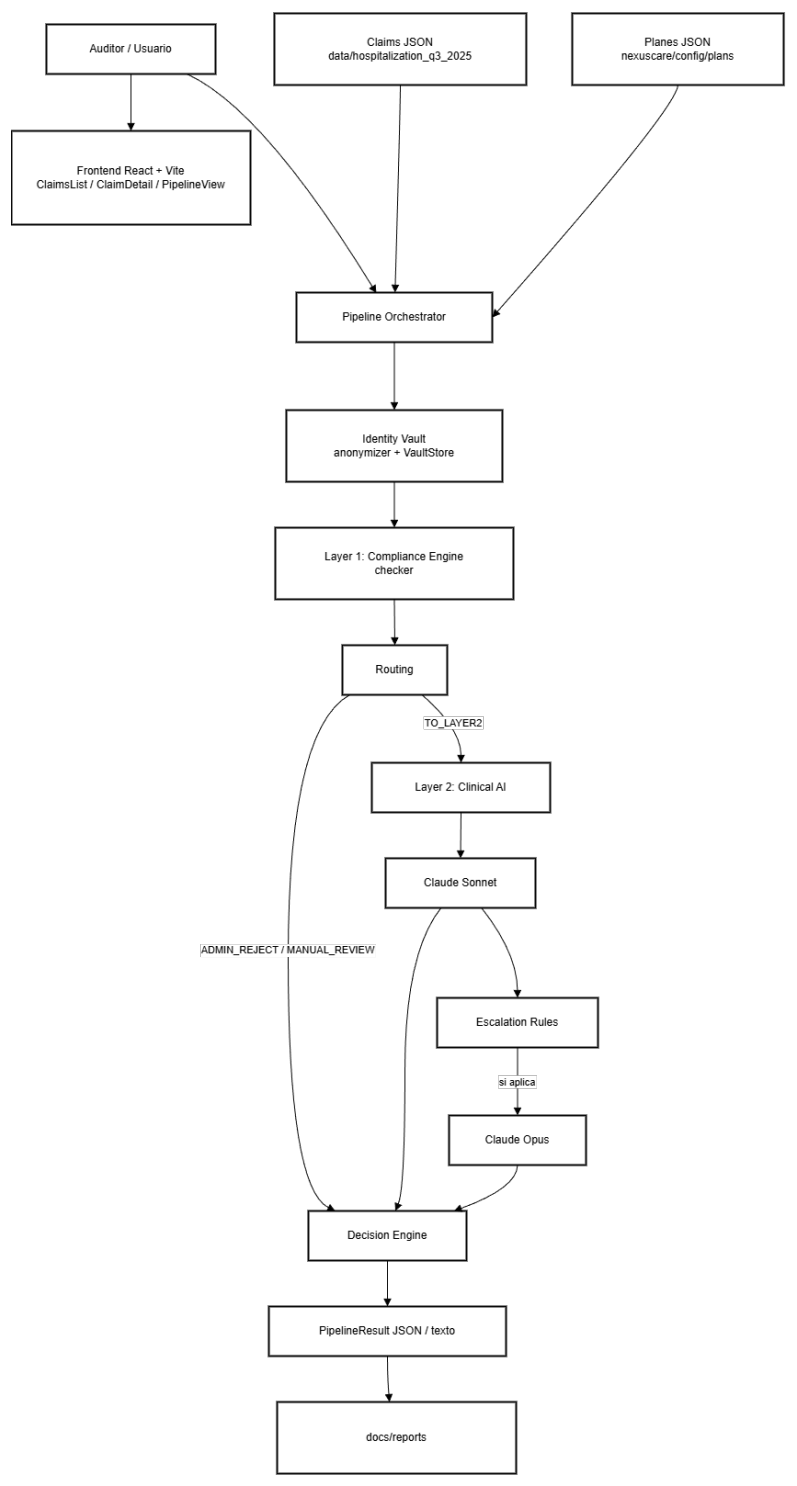
\includegraphics[width=0.96\textwidth,height=0.72\textheight,keepaspectratio]{images/p23_figure_1.png}
\caption{\textit{Workflow} del sistema: flujo de cinco fases desde la liquidación hasta la decisión del auditor.}
\label{fig:p23_figure_1}
\end{figure}

\begin{figure}[H]
\centering
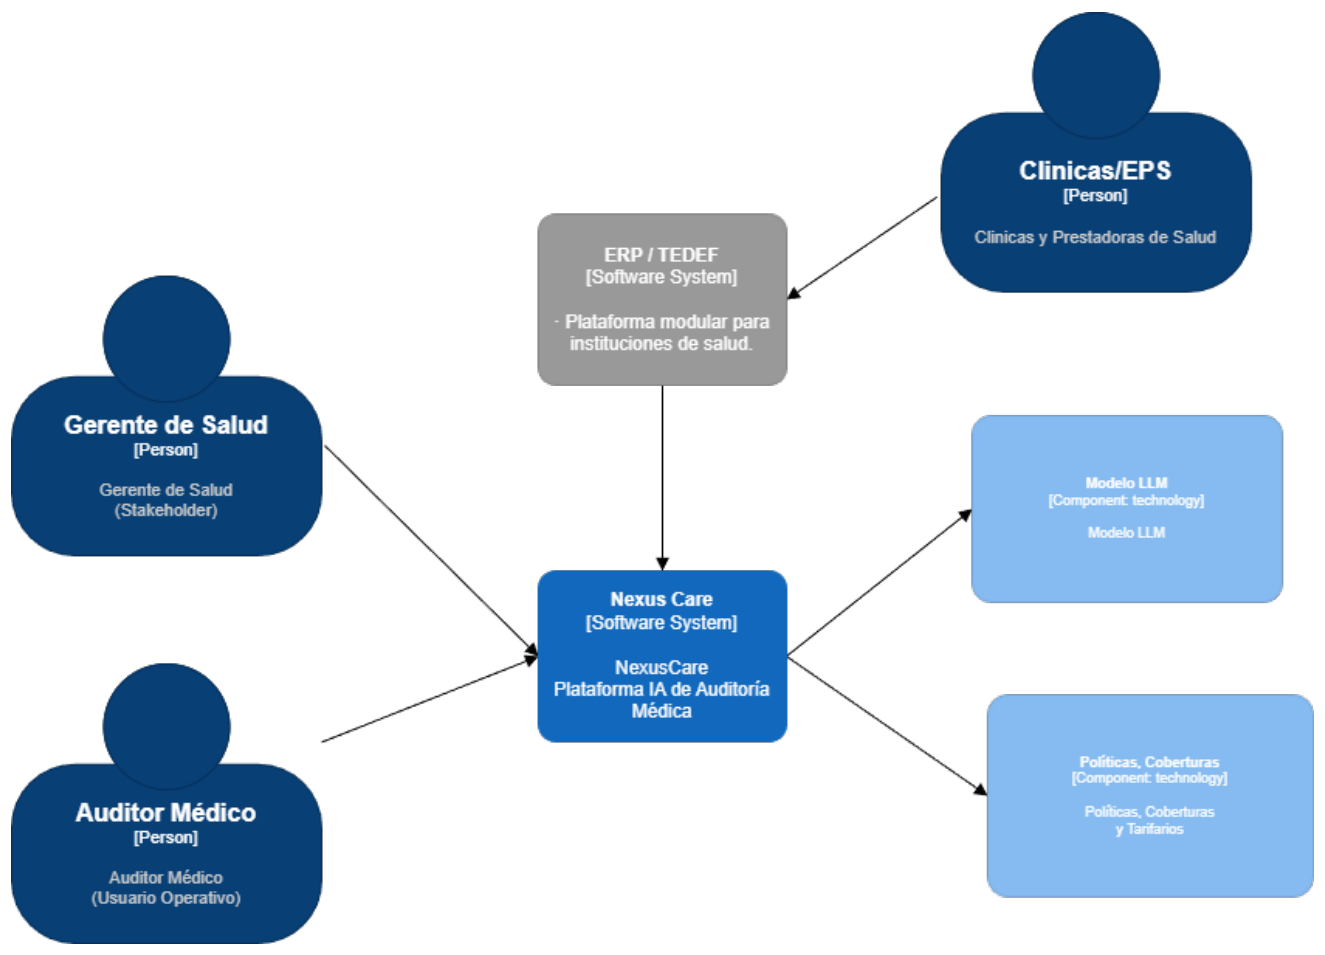
\includegraphics[width=0.96\textwidth,height=0.72\textheight,keepaspectratio]{images/p24_figure_1.png}
\caption{Diagrama C4 de contexto del problema: nivel 1 \cite{brown2018c4}.}
\label{fig:p24_figure_1}
\end{figure}

\begin{figure}[H]
\centering
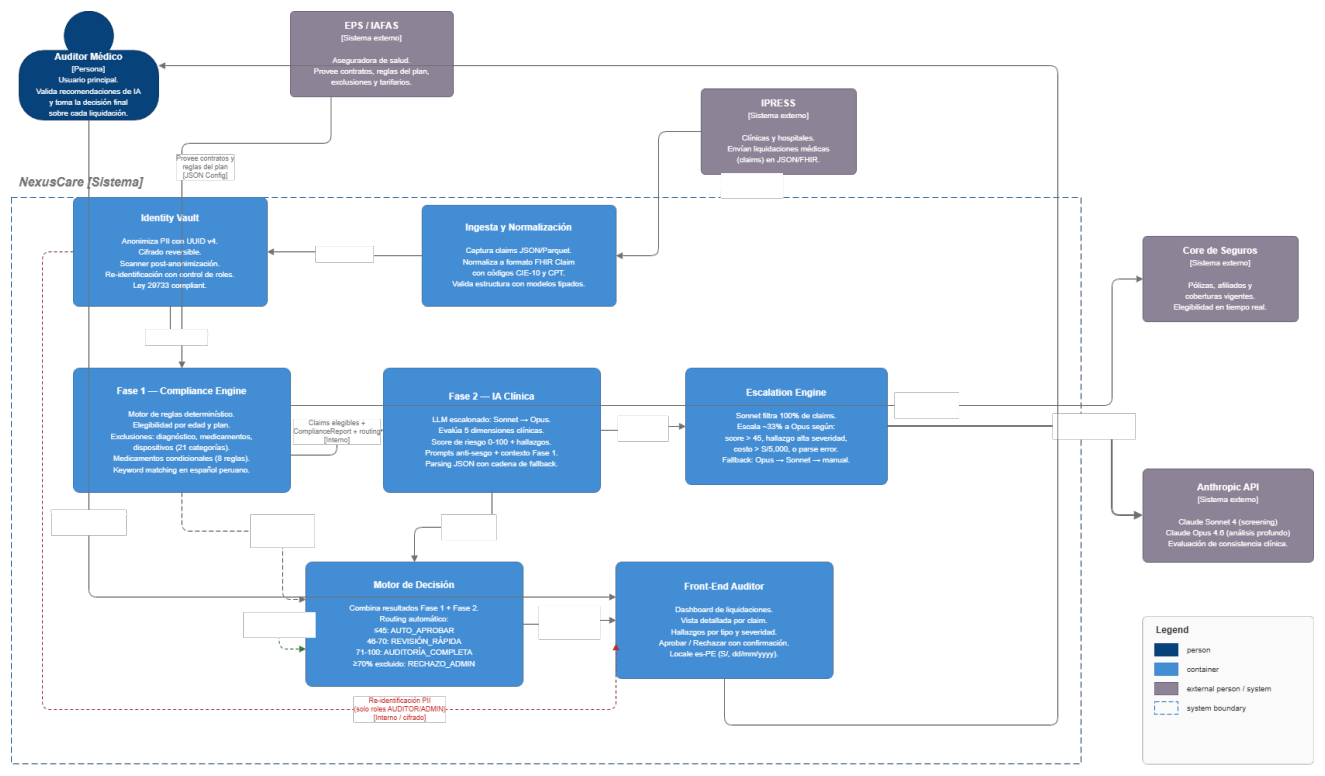
\includegraphics[width=0.96\textwidth,height=0.72\textheight,keepaspectratio]{images/p25_figure_1.png}
\caption{Diagrama C4 de contenedores del sistema.}
\label{fig:p25_figure_1}
\end{figure}

\section{Ingesta y normalización}

Las liquidaciones llegan como archivos JSON individuales, cada uno representando un caso hospitalario completo. La estructura incluye:
\begin{itemize}
     \item \textbf{Datos del paciente:}  nombre, edad, sexo (los dos últimos se preservan como quasi-identificadores necesarios para la validación clínica CIE-10).

     \item \textbf{Datos del prestador:} nombre del médico tratante (anonimizado) y especialidad.

    \item \textbf{Diagnóstico:} código CIE-10 y descripción textual.

    \item \textbf{Servicios:} organizados en siete categorías (farmacia, procedimientos, clínica, imagenología, consultas, laboratorio, otros servicios), cada una con una lista de ítems que incluyen código, descripción y costo.
     
\end{itemize}

La validación estructural se realiza mediante modelos Pydantic v2, definidos en nexuscare/compliance/models.py.

La clase \textit{Claim} y sus modelos anidados garantizan que toda liquidación procesada cumpla con el esquema esperado. Los principales modelos involucrados son Patient, Provider, Diagnosis, Services, ServiceCategory y ServiceItem.

Los costos se almacenan como strings para preservar el formato original y se convierten a float bajo demanda mediante la propiedad cost float de ServiceItem.

La fuente de datos del MVP consiste en 101 liquidaciones hospitalarias del Q3 2025 de MediVida, complementadas con registros proxy de pacientes (visitas únicas y múltiples) indexados por un catálogo maestro (patient index.json).

\section{\textit{Identity Vault}: protección de datos personales}

Antes de que cualquier dato llegue al LLM, el sistema ejecuta un proceso de anonimización que implementa los principios de \textit{privacy} by design establecidos en Capstone 1 \cite{hurtado2025nexuscare}, en cumplimiento con la Ley No 29733 \cite{peru2011ley29733} y alineado con los principios de minimización de datos del GDPR \cite{eu2024aiact}.

El módulo \textit{Identity Vault} (nexuscare/vault/) comprende cuatro componentes:

 \textbf{\textit{Anonymizer} (anonymizer.py)} Reemplaza los nombres de paciente y médico con identificadores UUID v4. El proceso es idempotente: la misma persona siempre recibe el mismo UUID, lo que permite correlacionar liquidaciones de un mismo paciente sin exponer su identidad. Los datos clínicos (diagnósticos, medicamentos, costos) no se anonimizan porque son necesarios para el análisis de consistencia.

 
 \textbf{\textit{Scanner} (scanner.py)} Detector de fugas de PII post-anonimización. Busca patrones específicos del contexto peruano: DNI (8 dígitos), números CMP (Colegio Médico del Perú), números
 \textbf{\textit{Vault Store} (store.py)} Almacenamiento persistente cifrado para los mapeos PII-UUID. Utiliza AES-256-GCM con derivación de clave mediante SHA-256 sobre la clave de entorno (VAULT\_KEY). Mantiene dos índices: anon\_id hacia PIIRecord (para re-identificación) y \textit{hash} del \textit{lookup key} hacia anon id (para anonimización idempotente).
telefónicos con prefijo +51, y direcciones de correo electrónico. Los UUID se excluyen del escaneo porque son valores esperados en datos anonimizados.

\textbf{\textit{Reidentifier} (reidentifier.py)} Servicio de re-identificación con control de acceso basado en roles. Solo los roles AUDITOR y ADMIN pueden resolver un UUID a la identidad real. Cada operación de re-identificación se registra en un log de auditoría inmutable (\textit{append-only}), cumpliendo el requisito de trazabilidad (RF5).

El flujo completo es: \textit{Claim}(PII) → Anonymize → \textit{Claim}(anon) → LLM → Result → Re-identify → Auditor. En ningún momento el LLM procesa datos que permitan identificar a un paciente o médico real.

\section{Fase 1: motor de reglas contractuales}

Fase 1 implementa la verificación determinística de cumplimiento contractual. Es la primera línea de filtrado y opera sin ningún componente de IA.

El motor está implementado en nexuscare/compliance/ y ejecuta cinco verificaciones secuenciales sobre cada liquidación:

\noindent \textbf{1. Elegibilidad por edad} Verifica que la edad del paciente se encuentre dentro del rango de ingreso permitido por el plan. Para MediVida Más 65, el rango es de 65 a 100 años; para MediVida Premium, de 0 a 64 años. Un paciente fuera del rango de su plan genera un \textit{finding EXCLUDED} en la categoría \textit{eligibility} y el \textit{claim} se envía a AUDITORIA COMPLETA, sin pasar por el LLM.

\noindent \textbf{2. Validación de diagnóstico} CIE-10 Consulta un catálogo CIE-10 embebido para verificar: (a) que el código diagnóstico existe, (b) que es consistente con el sexo del paciente, y (c) que es consistente con el rango de edad. Este módulo (cie10.py) realiza una búsqueda fuzzy para manejar variaciones en la codificación.


\noindent \textbf{3. Exclusiones por diagnóstico} Evalúa 21 exclusiones generales definidas en la configuración del plan, cada una con sus prefijos CIE-10 asociados. Las categorías incluyen: enfermedades congénitas (prefijo Q), accidentes laborales (Z57), deportes de riesgo (V, W, X, Y), abuso de sustancias (F10–F19, T40–T51), salud mental (F), cirugía estética y tratamientos de obesidad, entre otras. Algunas exclusiones tienen excepciones textuales que se preservan como \textit{findings} de tipo REVIEW\_NEEDED.
\noindent \textbf{4. Exclusiones de medicamentos} Verifica cada ítem de la farmacia contra 25 categorías de medicamentos excluidos (anticonceptivos, vitaminas, psicotrópicos, hormonoterapia, etc.) mediante \textit{keyword matching} con normalización de texto en español. También evalúa 8 medicamentos condicionales cuya cobertura depende del diagnóstico.

\noindent \textbf{5. Exclusiones de dispositivos e implantes} Verifica 26 \textit{keywords} de exclusión (prótesis, stents, marcapasos, etc.) frente a 37 \textit{keywords} de excepción (stents coronarios, placas y tornillos de traumatología, válvulas de derivación, etc.). La lógica distingue entre insumos médicos básicos y dispositivos que requieren verificación contractual.

La normalización de texto en español (matchers.py) maneja tildes, caracteres especiales y mayúsculas de forma consistente. Esto es necesario porque las descripciones de medicamentos e insumos en las liquidaciones peruanas emplean convenciones de escritura heterogéneas.

Las configuraciones de plan se extraen de los contratos de seguro reales en formato PDF utilizando un proceso semiautomático: un LLM genera una primera versión JSON a partir de secciones específicas del contrato (extract plan rules.py), y un auditor humano valida y corrige el resultado (validate extraction.py). Los archivos JSON resultantes se almacenan en nexuscare/config/plans/ y se versionan junto con el código.

\textbf{\textit{Routing} de Fase 1} El resultado de Fase 1 determina el siguiente paso:
\begin{itemize}
    \item Si el paciente no es elegible: AUDITORIA_COMPLETA (omite LLM).
    \item Si el 70 \% o más de los ítems están excluidos: RECHAZO_ADMINISTRATIVO (omite LLM).
    \item  En cualquier otro caso: TO_LAYER2 (envía a Fase 2 para evaluación clínica).
\end{itemize}

Este \textit{routing} permite ahorrar el costo del LLM cuando ya existe una determinación contractual clara.

\section{Fase 2: evaluación clínica con LLM}

La Fase 2 es el componente de inteligencia artificial del \textit{pipeline}. Evalúa la consistencia clínica del expediente y asigna un puntaje de riesgo explicable.

\textbf{Evolución desde Capstone 1} El prototipo usaba MedGemma-4B, un modelo de fundación médica de Google DeepMind \cite{google2025medgemma}, desplegado localmente. Los resultados fueron alentadores (93 \% de \textit{parsing} exitoso), pero el modelo presentaba limitaciones: un contexto de 8,192 \textit{tokens} insuficiente para liquidaciones con más de 100 ítems, y una tendencia a producir análisis superficiales en casos complejos.

Para Capstone 2, se realizó un \textit{benchmark} comparativo Tabla~\ref{tab:benchmark-modelos-fase2} de cinco modelos sobre las 101 liquidaciones del \textit{dataset}  (505 evaluaciones totales):

\begin{table}[H]
    \centering
    \caption{Benchmark comparativo de modelos para la Fase 2}
    \label{tab:benchmark-modelos-fase2}

    \footnotesize
    \setlength{\tabcolsep}{5pt}
    \renewcommand{\arraystretch}{1.2}

    \begin{tabular}{
        l
        c
        c
        c
        c
        c
    }
        \toprule
        \textbf{Modelo}
        & \shortstack{\textbf{\textit{Sigma score}}}
        & \textbf{Hallazgos/caso}
        & \shortstack{\textbf{Costo/caso}\\\textbf{(USD)}}
        & \shortstack{\textbf{Fast-track}\\\textbf{(\%)}}
        & \shortstack{\textbf{Latencia}\\\textbf{promedio}} \\
        \midrule

        Claude Sonnet 4 & 20.1 & 3.0 & USD 0.028 & 24.8\,\% & $\sim 17$ s \\
        Claude Opus 4.6 & 15.3 & 6.8 & USD 0.278 & 3.1\,\%  & $\sim 50$ s \\
        GPT-5.4          & 8.8  & 6.2 & USD 0.027 & 0.0\,\%  & $\sim 27$ s \\
        Gemini 2.5 Pro   & 12.2 & 3.5 & USD 0.018 & 1.0\,\%  & $\sim 38$ s \\
        MedGemma 27B     & 14.7 & 2.9 & USD 0.041 & 2.0\,\%  & Variable \\

        \bottomrule
    \end{tabular}
\end{table}

La desviación estándar del puntaje (\textit{sigma score}) mide la capacidad de discriminación del modelo: un sigma alto indica que el modelo diferencia entre casos de bajo y alto riesgo, mientras que un sigma bajo indica que asigna puntajes similares a todos los casos. Claude Sonnet 4 presentó la mayor discriminación ($\sigma$ = 20.1), con una distribución equilibrada entre las tres bandas de riesgo (25 \% bajo / 45 \% medio / 31 \% alto). GPT-5.4, con $\sigma$ = 8.8, asignó puntajes altos a prácticamente todas las liquidaciones (0 \% de \textit{fast-track}), lo que lo hace inviable para el caso de uso.

Claude Opus 4.6 generó el análisis clínico más profundo (6.8 hallazgos por caso, 682 totales), pero a un costo 10 veces mayor que Sonnet y con una tasa de \textit{fast-track} del 3.1 \%, lo que refleja una tendencia a sobrevalorar el riesgo.

Estos resultados motivaron la adopción de una estrategia escalonada, implementada en nexuscare/pipeline/escalate

\textbf{Paso 1:} Claude Sonnet 4 filtra el 100 \% de las liquidaciones ($\sim$17 segundos, \$0.028 por caso).

\textbf{Paso 2:} Se escala a Claude Opus 4.6 el $\sim$33 \% de los casos, según cuatro criterios: (a) puntaje de Sonnet > 45, (b) hallazgo de alta severidad de tipo inconsistencia clínica o sobrecosto, (c) costo total de la liquidación > S/5,000 con ítems en revisión, o (d) error de \textit{parsing} en la respuesta de Sonnet.

\textbf{\textit{Fallback}:} si Opus falla (error de parseo o \textit{timeout}), el sistema revierte al resultado de Sonnet.

El costo por liquidación con la estrategia escalonada es de $\sim$\$0.12, un 57 \% inferior al costo de usar Opus en todos los casos (\$0.278). Para un lote de 101 liquidaciones, el costo total de API fue de \$12.00, frente a \$28.08 con Opus en exclusiva.

\textbf{Ejemplo ilustrativo del benchmark} La liquidación H0710170 (obstrucción del conducto biliar, K83.1, 118 ítems, gastroenterología) fue evaluada por los cinco modelos. Claude Sonnet le asignó un puntaje de 70 e identificó 3 hallazgos. Claude Opus le asignó 75 puntos con 7 hallazgos, detectando la duplicidad terapéutica de inhibidores de bomba de protones y un patrón de reversiones en farmacia que sugiere problemas de control de inventario. Todos coincidieron en la inconsistencia principal: material endoscópico presente sin un procedimiento endoscópico registrado. Esta convergencia en el hallazgo principal, con divergencia en la profundidad del análisis complementario, justifica la estrategia escalonada.

\textbf{Dimensiones de evaluación clínica} El LLM evalúa cada liquidación en cinco dimensiones, definidas en el \textit{prompt} de auditoría (nexuscare/benchmark/prompts.py):

\noindent \textbf{1. Consistencia diagnóstico-procedimiento.}

\noindent \textbf{2. Consistencia diagnóstico-especialidad.}

\noindent \textbf{3. Protocolo farmacológico.}

\noindent \textbf{4. Materiales e insumos.}

\noindent \textbf{5. Puntaje de riesgo (0–100).}

La escala de producción utiliza cuatro bandas calibradas con el \textit{Golden Set}: 0–25 muy bajo, 26–45 bajo, 46–70 medio, 71–100 alto. Los hallazgos se tipifican en cuatro categorías: \textbf{Inconsistencia Clínica, Omisión, Sobrecosto y Duplicado.} Cada hallazgo lleva una severidad (alta, media, baja).

La salida del LLM se estructura como JSON con campos tipados, lo que permite al \textit{pipeline} procesarla de forma programática. El módulo de \textit{parsing} (extract json en run benchmark.py) maneja respuestas con bloques de código en \textit{Markdown}. Cuando el \textit{parsing} falla, el caso se marca como \textit{parse error} y se escala a Opus o se deriva a auditoría completa.

\section{Motor de decisión y \textit{routing}}

El módulo nexuscare/pipeline/decision.py combina los resultados de Fase 1 y Fase 2 para generar la recomendación final. Las reglas de decisión se encuentran en la Tabla~\ref{tab:reglas-decision-pipeline}:

\begin{table}[H]
    \centering
    \caption{Reglas de decisión del \textit{pipeline} integrado}
    \label{tab:reglas-decision-pipeline}

    \footnotesize
    \setlength{\tabcolsep}{8pt}
    \renewcommand{\arraystretch}{1.2}

    \begin{tabular}{
        p{0.62\textwidth}
        p{0.30\textwidth}
    }
        \toprule
        \textbf{Condición}
        & \textbf{Decisión} \\
        \midrule

        Fase 1: 100\,\% de cobertura + Fase 2:
        \textit{score} $\leq 45$
        & \texttt{FAST\_TRACK} \\

        Fase 1: $\geq 70\,\%$ de ítems excluidos
        & \texttt{RECHAZO\_ADMINISTRATIVO} \\

        Fase 2: \textit{score} entre 46 y 70
        & \texttt{REVISION\_RAPIDA} \\

        Fase 2: \textit{score} $> 70$
        & \texttt{AUDITORIA\_COMPLETA} \\

        Fase 1: ítems condicionales + Fase 2:
        \textit{score} entre 31 y 45
        & \texttt{REVISION\_RAPIDA} \\

        Paciente no elegible
        & \texttt{AUDITORIA\_COMPLETA} \\

        \bottomrule
    \end{tabular}
\end{table}

Los umbrales (45, 70) se calibraron utilizando el \textit{Golden Set} de 17 liquidaciones curadas. La calibración apunta a una tasa de \textit{fast-track} del 65 \%, confirmada por la ejecución del \textit{pipeline} integrado. Los tres mecanismos de calibración son:

\noindent \textbf{1. Pre-filtrado de Fase 1:} la eliminación de exclusiones contractuales antes del LLM reduce los falsos positivos del modelo.

\noindent \textbf{2. Umbrales recalibrados:} los puntos de corte se ajustan con el \textit{Golden Set} para maximizar la tasa de \textit{fast-track} sin degradar la detección de casos de alto riesgo.

\noindent \textbf{3. \textit{Prompts} anti-sesgo:} instrucciones explícitas al LLM para evitar la sobre-penalización de liquidaciones rutinarias.

\section{\textit{Front-end} del auditor}

La interfaz de validación del auditor se implementó como una aplicación de página única (SPA) utilizando React 19, TypeScript 5.9, Vite 8, Tailwind CSS 4 y React Router 7.

La aplicación consta de tres vistas principales:

\textbf{ClaimsList (\textit{Dashboard})} Tabla interactiva que muestra todas las liquidaciones del lote evaluado, con columnas para: ID del expediente, paciente (anonimizado), diagnóstico, especialidad, monto total, puntaje de riesgo, estado de la recomendación, y fecha. Soporta búsqueda por texto libre, filtros por estado y ordenamiento por cualquier columna.

\textbf{ClaimDetail (Revisión)} Vista de detalle de una liquidación individual. Presenta los datos del paciente y diagnóstico, los resultados de Fase 1, los resultados de Fase 2 y la tabla completa de ítems facturados con indicación visual de los que fueron marcados como cuestionables. Incluye botones de Aprobar y Rechazar con diálogo de confirmación, implementando el \textit{override} humano requerido por RF8.

\textbf{PipelineView} Visualización interactiva del \textit{pipeline} de cinco fases, con simulación paso a paso que permite al auditor, o a un \textit{stakeholder} no técnico, comprender el flujo de procesamiento de una liquidación.

Toda la interfaz utiliza texto en español y formatos de moneda y fecha correspondientes a la configuración regional es-PE. Los componentes reutilizables (FindingCard, RiskBadge, StatusBadge) encapsulan la lógica de presentación visual de hallazgos, puntajes y estados.

Interfaz del auditor: vista de detalle de una liquidación (ClaimDetail).

\begin{figure}[H]
\centering
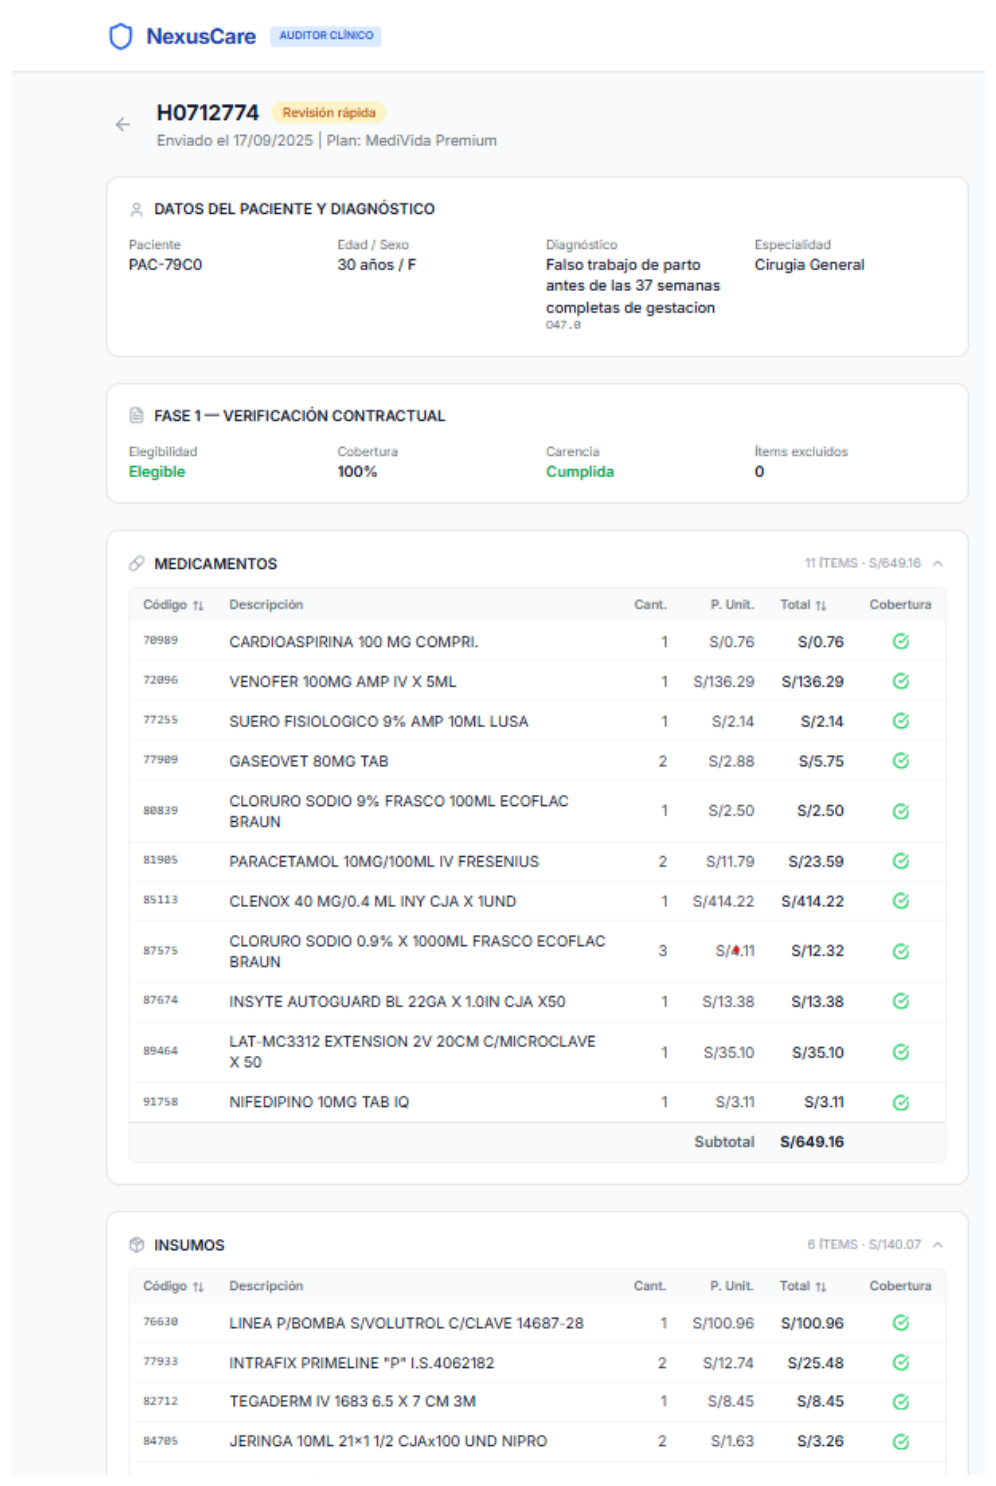
\includegraphics[width=0.96\textwidth,height=0.72\textheight,keepaspectratio]{images/p33_figure_1.png}
\caption{Interfaz del auditor: vista detallada de una liquidación.}
\end{figure}

\section{\textit{Stack} tecnológico}


\begin{table}[H]
    \centering
    \caption{\textit{Stack} tecnológico de NexusCare}
    \label{tab:stack-tecnologico-nexuscare}

    \footnotesize
    \setlength{\tabcolsep}{8pt}
    \renewcommand{\arraystretch}{1.3}

    \begin{tabular}{
        p{0.27\textwidth}
        p{0.65\textwidth}
    }
        \toprule
        \textbf{Capa}
        & \textbf{Tecnología} \\
        \midrule

        \textit{Backend} / \textit{Pipeline}
        & Python 3.11, Pydantic v2, Anthropic SDK y \textit{httpx}. \\

        \textit{Frontend}
        & React 19, TypeScript 5.9, Vite 8, Tailwind CSS 4,
          React Router 7 y \textit{lucide-react}. \\

        Datos
        & JSON (liquidaciones), Parquet (datos crudos) y CIE-10
          (catálogo embebido). \\

        Testing
        & \textit{pytest}, con 190 funciones de prueba distribuidas
          en siete archivos. \\

        Privacidad
        & AES-256-GCM, PBKDF2 para derivación de claves y UUID v4
          para anonimización. \\

        IA
        & Claude Sonnet 4 para \textit{screening} y Claude Opus 4.6
          para análisis profundo. \\

        Diagramas
        & PlantUML C4 y \textit{python-pptx}. \\

        \bottomrule
    \end{tabular}
\end{table}

\section{Decisiones de diseño y \textit{trade-offs}}

\noindent \textbf{1. Arquitectura de dos fases vs. LLM único} Fase 1 (reglas) + Fase 2 (IA) permite que las verificaciones contractuales sean determinísticas, reproducibles y auditables. El \textit{trade-off} es la complejidad adicional de mantener dos subsistemas sincronizados y las configuraciones de plan actualizadas.

\noindent \textbf{2. Estrategia escalonada de modelos vs. modelo único} La combinación Sonnet (\textit{screening}) + Opus (análisis profundo) reduce el costo en un 57 \% respecto a usar Opus en todos los casos, con una pérdida marginal en la profundidad de análisis en los casos de bajo riesgo. El \textit{trade-off} radica en la complejidad de la lógica de escalación.

\noindent \textbf{3. Extracción de reglas de plan mediante LLM + validación humana} Los contratos de seguro son documentos PDF complejos, con lenguaje legal y estructuras variadas entre los planes. La extracción automatizada mediante LLM reduce el tiempo de configuración de días a horas, pero requiere validación humana para garantizar la precisión.

\noindent \textbf{4. \textit{Human-in-the-loop} obligatorio} El sistema nunca toma la decisión final en casos de riesgo medio o alto. La contrapartida es clara: la ganancia de eficiencia queda acotada al segmento de bajo riesgo.

\noindent \textbf{5. \textit{Privacy} by design: PII nunca llega al LLM} Los datos personales se anonimizan antes de enviar cualquier información al modelo y se reidentifican únicamente en el entorno local del auditor, con control de acceso y registro de auditoría.

\section{Resultados preliminares y proyecciones}
\label{sec:resultados-preliminares}

Los resultados del benchmark y las pruebas con el pipeline integrado permiten estimar el desempeño proyectado del sistema en producción.

\textbf{Cobertura de procesamiento} El pipeline procesó exitosamente las 101 liquidaciones del \textit{dataset}  sin errores fatales. La validación estructural con Pydantic v2 no rechazó ningún caso. Los 190 \textit{tests} automatizados cubren el motor de reglas, el pipeline integrado, la lógica de escalación, el \textit{vault} de identidad, el \textit{Golden Set} y la integración \textit{end-to-end}.

\textbf{Distribución de decisiones proyectada} Con los umbrales calibrados y el pre-filtrado de Fase 1, la distribución proyectada para un lote típico de 101 liquidaciones hospitalarias es:

\begin{table}[H]
    \centering
    \caption{Distribución proyectada de decisiones por categoría}
    \label{tab:distribucion-proyectada-decisiones}

    \footnotesize
    \setlength{\tabcolsep}{7pt}
    \renewcommand{\arraystretch}{1.25}

    \begin{tabular}{
        p{0.30\textwidth}
        p{0.18\textwidth}
        p{0.44\textwidth}
    }
        \toprule
        \textbf{Categoría}
        & \textbf{\% proyectado}
        & \textbf{Tiempo estimado de auditoría} \\
        \midrule

        \texttt{FAST\_TRACK}
        & 55--65\,\%
        & $\sim 1$ minuto de verificación visual por caso. \\

        \texttt{REVISION\_RAPIDA}
        & 15--20\,\%
        & $\sim 10$ minutos por caso (revisión focalizada). \\

        \texttt{AUDITORIA\_COMPLETA}
        & 10--15\,\%
        & $\sim 45$ minutos por caso (auditoría profunda). \\

        \texttt{RECHAZO\_ADMINISTRATIVO}
        & 3--5\,\%
        & $\sim 2$ minutos por caso (verificación administrativa). \\

        \bottomrule
    \end{tabular}
\end{table}
Con estos números, el tiempo total del lote se proyecta en 16 horas frente a las 75.8 horas del proceso manual, una reducción del 79 \%.

\textbf{Estimación de costos operativos} El costo de API por lote de 101 liquidaciones, con la estrategia escalonada, fue de \$12.00. Es menos del 0.01 \% del valor promedio de un lote hospitalario.

\textbf{Limitaciones observadas} La principal limitación identificada es la tendencia del LLM a generar hallazgos sobre inconsistencias documentales que pueden ser normales en el flujo operativo de la IPRESS pero que el modelo interpreta como señales de riesgo. Otra limitación es la dependencia de APIs externas para el componente de Fase 2.

\addcontentsline{toc}{section}{CAPÍTULO VIII}
\chapter{DESARROLLO Y CONSTRUCCIÓN}

\section{Cronología de desarrollo}

El desarrollo de \textbf{NexusCare} abarca dos ciclos académicos con objetivos y entregables distintos.

\textbf{Capstone 1 (agosto–diciembre 2025)} produjo un prototipo de concepto basado en MedGemma- 4B, un modelo de fundación médica de 4 mil millones de parámetros desarrollado por Google DeepMind. El modelo se desplegó localmente y procesó 101 liquidaciones hospitalarias con una tasa de \textit{parsing} exitoso del 93 \% (7 casos fallaron por límite de contexto). El prototipo validó parcialmente tres hipótesis técnicas: que un LLM puede generar análisis clínicos estructurados sobre liquidaciones, que el tiempo de procesamiento se reduce de 45 a menos de 5 minutos por caso, y que la generación de puntajes de riesgo con justificaciones textuales es técnicamente viable. Sin embargo, el prototipo dejó abiertas tres brechas que definieron la hoja de ruta de Capstone 2: la calibración del modelo, la ausencia de verificación contractual y la falta de protección de datos personales.

\textbf{Capstone 2 (enero–marzo 2026)} reconstruyó el sistema desde la arquitectura. El cambio más significativo fue abandonar MedGemma-4B como modelo único y adoptar una arquitectura de dos fases con múltiples modelos. La primera decisión fue separar la verificación contractual (Fase 1) del análisis clínico (Fase 2), motivada por la observación de que MedGemma confundía exclusiones contractuales con inconsistencias clínicas. La segunda fue realizar un \textit{benchmark} comparativo de cinco modelos para seleccionar la combinación óptima basándose en datos, no en supuestos. La tercera fue construir un \textit{Identity Vault} para anonimización de PII antes de enviar datos al LLM, en cumplimiento con la Ley 29733.

La cronología del desarrollo fue la siguiente. En enero, el foco estuvo en el motor de reglas contractuales (nexuscare/compliance/) y en la extracción semiautomática de configuraciones de plan a partir de los contratos en formato PDF de MediVida. Febrero fue el mes más intenso: se ejecutó el benchmark de cinco modelos (505 evaluaciones), se diseñó la estrategia escalonada

Sonnet+Opus y se implementó el \textit{pipeline} integrado con orquestador, escalación y motor de decisión. El último mes se dedicó a la calibración (el \textit{Golden Set} de 17 liquidaciones, los umbrales de decisión) y a la interfaz React del auditor.

Dos decisiones de diseño fueron descartadas durante el proceso. La primera fue el despliegue de MedGemma 27B en un \textit{endpoint} de Vertex AI con GPU A100: aunque funcionó técnicamente, el modelo demostró menor capacidad de discriminación que Claude Sonnet y un \textit{throughput} inferior, con un costo comparable. El \textit{endpoint} se desmanteló tras el benchmark. La segunda fue un módulo de detección de fraude basado en patrones de prescripción por médico, que requería acceso a datos de identidad del médico tratante, incompatible con la decisión de \textit{privacy by design}  adoptada en la sección 7.3.

La siguiente tabla~\ref{tab:cronologia-desarrollo} resume la cronología de iteraciones:

\begin{table}[H]
    \centering
    \caption{Cronología de iteraciones del desarrollo}
    \label{tab:cronologia-desarrollo}

    \scriptsize
    \setlength{\tabcolsep}{4pt}
    \renewcommand{\arraystretch}{1.25}

    \begin{tabular}{
        p{0.14\textwidth}
        p{0.12\textwidth}
        p{0.19\textwidth}
        p{0.34\textwidth}
        p{0.15\textwidth}
    }
        \toprule
        \textbf{Fase}
        & \textbf{Periodo}
        & \textbf{Foco principal}
        & \textbf{Entregables clave}
        & \textbf{Decisiones descartadas} \\
        \midrule

        Capstone 1
        & Ago.--dic. 2025
        & Prototipo MedGemma-4B
        & 101 liquidaciones procesadas, 93\,\% de éxito y tres
          hipótesis validadas.
        & --- \\

        Capstone 2, ene.
        & Ene. 2026
        & Motor de reglas contractuales
        & Módulo \texttt{compliance/} y extracción de planes desde
          PDF hacia JSON.
        & --- \\

        Capstone 2, feb.
        & Feb. 2026
        & Benchmark y pipeline
        & 505 evaluaciones, estrategia escalonada Sonnet + Opus
          y orquestador.
        & \textit{Endpoint} MedGemma 27B. \\

        Capstone 2, mar.
        & Mar. 2026
        & Calibración e interfaz
        & \textit{Golden Set} de 17 \textit{claims}, umbrales de
          decisión e interfaz React para el auditor.
        & Módulo de detección de fraude. \\

        \bottomrule
    \end{tabular}
\end{table}
\section{Dataset y preparación}

El \textit{dataset}  del MVP consiste en 101 liquidaciones hospitalarias del Q3 2025 de MediVida, almacenadas como archivos JSON individuales en data/hospitalization q3 2025/. Los datos originales provienen de la plataforma TEDEF en formato Parquet (cabecera.parquet, detalle all.parquet), que se transformaron a JSON normalizado durante Capstone 1. Cada liquidación contiene entre 5 y 368 ítems de servicio, con un promedio de S/21,840 por caso.

La anonimización se implementó en dos niveles. A nivel de \textit{dataset} , el nombre de la IAFAS fue sustituido por un seudónimo (MediVida) desde la fase de preparación de datos. A nivel de pipeline, el \textit{Identity Vault} sustituye los nombres de pacientes y médicos por identificadores UUID

v4 antes de cada invocación al LLM, manteniendo la edad y el sexo como cuasiidentificadores requeridos para la validación clínica de códigos CIE-10.

Los registros proxy de pacientes (data/proxy records q3 2025/) complementan las liquidaciones con información de contexto clínico: visitas previas del paciente (single visit/ para pacientes con una sola atención, multi visit/ para pacientes con historial), indexados mediante patient index.json. Estos registros permiten al sistema evaluar si una hospitalización es un evento aislado o parte de una condición crónica, lo que influye en la evaluación de consistencia clínica.

\section{Construcción del \textit{Golden Set}}

El \textit{Golden Set} es un conjunto curado de 17 liquidaciones con clasificaciones esperadas, definido en nexuscare/pipeline/golden set.py. Su función es doble: regresión y calibración de umbrales. Es importante notar que el \textit{Golden Set} no constituye un conjunto de validación independiente: los umbrales de decisión (45, 70) se calibraron usando estos mismos 17 casos, por lo que su uso posterior para evaluar esos umbrales tiene circularidad inherente. Su valor radica en la regresión continua.

La selección de las 17 liquidaciones siguió criterios deliberados para cubrir los escenarios representativos del pipeline:

\textbf{10 candidatas a \textit{fast-track}} Liquidaciones rutinarias con cobertura completa (> 95 \%), pacientes elegibles y diagnósticos consistentes con los servicios facturados. Se seleccionaron para cubrir diversidad de especialidades, incluyendo traumatología, medicina interna, cirugía general, pediatría, gastroenterología, neumología y nefrología.

\textbf{2 casos complejos pero consistentes} Liquidaciones con alto número de ítems donde la expectativa es FAST_TRACK o REVISION_RAPIDA. Estos casos prueban que el LLM no penaliza por volumen cuando la consistencia clínica es adecuada.

\textbf{2 casos con ítems condicionales} Liquidaciones de urología con medicamentos cuya cobertura depende del diagnóstico. Validan que el \textit{routing} de ítems condicionales funciona correctamente.

\textbf{3 casos geriátricos de alta complejidad} Pacientes de 81, 89 y 99 años en el plan Más 65. Estos casos validan que el sistema no penaliza por edad cuando la cobertura contractual es completa.

Las clasificaciones esperadas de las 17 liquidaciones fueron validadas por un auditor médico con experiencia en liquidaciones hospitalarias. Una limitación del \textit{Golden Set} es que las clasificaciones fueron definidas por un único auditor, por lo que no es posible calcular acuerdo interevaluador.

Cada entrada del \textit{Golden Set} especifica el \textit{routing} esperado de Fase 1, el estado de elegibilidad, el ratio mínimo de cobertura, el puntaje máximo aceptable de Fase 2 y la decisión final esperada. Los \textit{tests} automatizados en tests/test golden set.py verifican estas expectativas.

La composición completa del \textit{Golden Set} se detalla en la siguiente tabla~\ref{tab:composicion-golden-set}:

\begin{table}[H]
    \centering
    \caption{Composición del \textit{Golden Set}}
    \label{tab:composicion-golden-set}

    \scriptsize
    \setlength{\tabcolsep}{3.5pt}
    \renewcommand{\arraystretch}{1.15}

    \begin{tabular}{
        c
        l
        p{0.23\textwidth}
        c
        c
        l
        p{0.22\textwidth}
    }
        \toprule
        \textbf{\#}
        & \textbf{claim\_id}
        & \textbf{Especialidad}
        & \textbf{Edad}
        & \textbf{Ítems}
        & \textbf{Plan}
        & \textbf{Decisión esperada} \\
        \midrule

        1  & H0710606 & Traumatología y Ortopedia & 70 & 133 & \texttt{mas\_65} & \texttt{FAST\_TRACK} \\
        2  & H0710688 & Traumatología y Ortopedia & 70 & 5   & \texttt{mas\_65} & \texttt{FAST\_TRACK} \\
        3  & H0710710 & Medicina Interna           & 79 & 127 & \texttt{mas\_65} & \texttt{FAST\_TRACK} \\
        4  & H0710288 & Pediatría                   & 3  & 14  & \texttt{premium} & \texttt{FAST\_TRACK} \\
        5  & H0710396 & Medicina Interna            & 33 & 26  & \texttt{premium} & \texttt{FAST\_TRACK} \\
        6  & H0710206 & Traumatología               & 55 & 50  & \texttt{premium} & \texttt{FAST\_TRACK} \\
        7  & H0710871 & Cirugía General             & 39 & 139 & \texttt{premium} & \texttt{FAST\_TRACK} \\
        8  & H0710170 & Gastroenterología           & 58 & 118 & \texttt{premium} & \texttt{FAST\_TRACK} \\
        9  & H0711614 & Neumología                  & 42 & 73  & \texttt{premium} & \texttt{FAST\_TRACK} \\
        10 & H0711305 & Nefrología                   & 77 & 53  & \texttt{mas\_65} & \texttt{FAST\_TRACK} \\
        11 & H0710712 & Neurocirugía                 & 34 & 310 & \texttt{premium} & \texttt{FAST\_TRACK / REVISION} \\
        12 & H0711699 & Cirugía Cardiovascular       & 75 & 252 & \texttt{mas\_65} & \texttt{FAST\_TRACK / REVISION} \\
        13 & H0710636 & Urología                     & 56 & 149 & \texttt{premium} & \texttt{FAST\_TRACK / REVISION} \\
        14 & H0712022 & Urología                     & 65 & 118 & \texttt{mas\_65} & \texttt{FAST\_TRACK / REVISION} \\
        15 & H0710235 & ---                          & 81 & --- & \texttt{mas\_65} & \texttt{FAST\_TRACK / REVISION} \\
        16 & H0710395 & ---                          & 89 & --- & \texttt{mas\_65} & \texttt{FAST\_TRACK / REVISION} \\
        17 & H0710770 & ---                          & 99 & 276 & \texttt{mas\_65} & \texttt{FAST\_TRACK / REVISION} \\

        \bottomrule
    \end{tabular}
\end{table}

\section{Proceso de benchmark}

El benchmark se ejecutó mediante el módulo nexuscare/benchmark/run benchmark.py. Las 101 liquidaciones fueron evaluadas por los cinco modelos, generando 505 evaluaciones individuales.

La ejecución se paralelizó por modelo dentro de cada liquidación: para cada caso, los cinco modelos se invocaron simultáneamente mediante ThreadPoolExecutor(max workers=5), donde cada worker ejecuta una llamada HTTP independiente a la API del modelo correspondiente. La paralelización redujo el tiempo total del benchmark de aproximadamente 14 horas en una ejecución secuencial a cerca de 4 horas.

Los parámetros de ejecución fueron: temperatura 0.1 para todos los modelos, max \textit{tokens} de 4,096 para los modelos de API y 2,048 para MedGemma, limitado por su contexto de 8,192 \textit{tokens}. MedGemma 27B se ejecutó en un \textit{endpoint} de Vertex AI con GPU A100 de 80 GB, utilizando el formato condensado del \textit{prompt}.


El \textit{parsing} de respuestas utilizó una cadena de \textit{fallback} implementada en extract json(): primero intenta un \textit{parsing} JSON directo; si falla, elimina las cercas de \textit{Markdown}; si eso también falla, busca el primer objeto JSON válido mediante \textit{regex}. Los resultados se almacenaron en un JSON consolidado con metadatos de ejecución y en archivos de texto individuales por \textit{claim} y modelo para inspección manual.
La configuración por modelo se resume en la siguiente tabla~\ref{tab:configuracion-benchmark-modelos}:

\begin{table}[H]
    \centering
    \caption{Configuración del benchmark por modelo}
    \label{tab:configuracion-benchmark-modelos}

    \footnotesize
    \setlength{\tabcolsep}{5pt}
    \renewcommand{\arraystretch}{1.2}

    \begin{tabular}{
        p{0.18\textwidth}
        p{0.16\textwidth}
        p{0.12\textwidth}
        p{0.10\textwidth}
        p{0.13\textwidth}
        p{0.23\textwidth}
    }
        \toprule
        \textbf{Modelo}
        & \textbf{Proveedor}
        & \textbf{max\_tokens}
        & \textbf{\textit{timeout}}
        & \textbf{Temperatura}
        & \textbf{Notas} \\
        \midrule

        Claude Sonnet 4
        & Anthropic API
        & 4,096
        & 120 s
        & \textit{default}
        & Modelo de \textit{screening}. \\

        Claude Opus 4.6
        & Anthropic API
        & 4,096
        & 180 s
        & \textit{default}
        & Análisis profundo. \\

        GPT-5.4
        & OpenAI API
        & 4,096
        & 180 s
        & \textit{default}
        & \texttt{max\_completion\_tokens}. \\

        Gemini 2.5 Pro
        & Google AI Studio
        & 8,192
        & 180 s
        & 0.1
        & --- \\

        MedGemma 27B
        & Vertex AI (A100)
        & 2,048
        & 300 s
        & 0.1
        & \textit{Prompt} condensado. \\

        \bottomrule
    \end{tabular}
\end{table}

\section{Iteraciones de \textit{prompt engineering}}

El diseño del \textit{prompt} clínico evolucionó entre tres versiones con diferencias sustantivas.

\textbf{\textit{Prompt} del benchmark} Definía al modelo como “auditor médico experto en seguros de salud en Perú” y solicitaba un informe JSON con cinco secciones: consistencia diagnóstico-procedimiento, consistencia diagnóstico-especialidad, protocolo farmacológico, materiales e insumos, y hallazgos críticos. La escala de riesgo original del benchmark usaba tres bandas: 0–30 (bajo), 31–60 (medio), 61–100 (alto). El \textit{prompt} instruye responder solamente con el JSON, lo que redujo los errores de \textit{parsing} a menos del 3 \%.

\textbf{\textit{Prompt} de producción} Incorpora tres cambios respecto al \textit{prompt} del benchmark. Primero, la instrucción anti-sesgo más relevante del sistema: “La verificación de cobertura contractual ya fue realizada por el sistema de reglas (Capa 1). Tu rol es exclusivamente la evaluación clínica.” Segundo, se inyecta el contexto de Fase 1 directamente en el \textit{prompt}: estado de elegibilidad, porcentaje de cobertura, número de exclusiones detectadas y detalle de cada exclusión. Tercero, la escala de riesgo se recalibró a cuatro bandas: 0–25 (muy bajo), 26–45 (bajo), 46–70 (medio), 71–100 (alto).

Las guías de calibración del \textit{prompt} de producción contienen instrucciones negativas explícitas para evitar penalizar complejidad clínica inherente, volumen de ítems y medicamentos genéricos estándar cuando son clínicamente consistentes.

\textbf{\textit{Prompt} de Opus para escalación} Define al modelo como “auditor médico SENIOR” y le proporciona el resultado previo de Sonnet. La instrucción clave es que puede confirmar, ajustar o descartar los hallazgos de Sonnet. Este diseño convierte a Opus en un revisor de segundo nivel, no en un evaluador independiente que repite el análisis desde cero.

\addcontentsline{toc}{section}{CAPÍTULO IX}
\chapter{MÉTRICA PRINCIPAL DE VALIDACIÓN}

\section{Definición}

La métrica principal del MVP es la \textbf{tasa de \textit{fast-track}:} el porcentaje de liquidaciones hospitalarias que el sistema evalúa, clasifica como de bajo riesgo y presenta al auditor con una recomendación fundamentada que este puede validar en aproximadamente 1 minuto. La meta es alcanzar una tasa del 50–60 \%. El rango de 50–60 \% representa la banda de operación óptima estimada. Una tasa inferior al 50 \% indicaría un impacto operativo insuficiente. Una tasa superior al 60 \% pero inferior al 75 \% es aceptable si no se observa un incremento en la tasa de falsos negativos, ya que implica que el sistema está liberando más capacidad del auditor de la inicialmente prevista.

Esta métrica refleja directamente la propuesta de valor de \textbf{\textit{NexusCare}}. Una tasa de \textit{fast-track} del 55 \% significa que, de un lote de 101 liquidaciones, aproximadamente 56 se resuelven en alrededor de 1 minuto cada una, lo que libera al auditor para concentrarse en los casos restantes que requieren un análisis profundo. El impacto operativo se mide a nivel de lote porque así opera el auditor: el valor se materializa cuando un lote completo se cierra más rápido, no cuando un caso aislado se procesa en menos tiempo.

La línea base se estableció durante Capstone 1: un lote de 101 liquidaciones hospitalarias requiere 75.8 horas de trabajo manual, aproximadamente 45 minutos por caso. La cifra de 45 minutos proviene de entrevistas con auditores médicos de MediVida durante Capstone 1, quienes reportaron un rango de 30 a 45 minutos para las liquidaciones hospitalarias, según la complejidad del caso. Se adoptó el extremo superior como supuesto conservador; no se midió mediante un estudio formal de tiempo y movimiento. Con una tasa de \textit{fast-track} del 55–60 \%, el tiempo total por lote se reduce a un rango estimado de 28 a 35 horas, equivalente a una reducción del 40–60 \%, según el tiempo efectivo que el auditor dedique a los casos de revisión rápida y a la auditoría completa.

\section{Métricas secundarias}

 \textbf{Tasa de falsos negativos (umbral máximo: 2 \%)} Mide el porcentaje de liquidaciones de riesgo medio o alto que el sistema clasifica incorrectamente como de bajo riesgo y recomienda para \textit{fasttrack}. A diferencia de los falsos positivos, que generan ineficiencia operativa, un falso negativo implica que una liquidación con inconsistencias clínicas o indicios de fraude pasa con una revisión mínima del auditor. Es la métrica de seguridad más crítica del sistema. El umbral del 2 \% se define como requisito no negociable: por encima de ese nivel, el riesgo regulatorio y reputacional para la aseguradora supera el beneficio operativo. Su medición precisa requiere un piloto con auditor real; en el alcance del MVP se estima indirectamente a partir del \textit{Golden Set}.

\textbf{Tasa de falsos positivos} Corresponde a liquidaciones clasificadas incorrectamente como de alto riesgo que, tras revisión del auditor, resultan ser casos rutinarios. Los falsos positivos tienen un costo operativo directo y un costo de confianza. Esta métrica solo puede medirse con precisión en un piloto con auditor real; en el alcance del MVP se estima a partir del \textit{Golden Set}.

\textbf{Concordancia auditor-sistema} Es el porcentaje de veces que el auditor acepta la recomendación del sistema sin modificarla. Valida el supuesto crítico de adopción y confianza. La interfaz React registra las acciones del auditor para calcular esta métrica en producción.

\textbf{Tiempo total por lote} Es un KPI derivado de la tasa de \textit{fast-track} y del tiempo de revisión de los casos no \textit{fast-track}. Se estima multiplicando el número de casos en cada categoría por el tiempo de revisión correspondiente. La meta es una reducción de al menos el 40 \% respecto a la línea base de 75.8 horas. Esta meta es conservadora: asume que todos los casos de auditoría completa siguen tomando 45 minutos y que los de revisión rápida toman 10 minutos. Si el auditor desarrolla confianza en el sistema y reduce el tiempo de los casos de revisión rápida, la reducción real podría superar el 60 \%.

\section{Método de medición}

La validación del MVP se basa en simulación y proyección, no en medición directa con un auditor en producción. Esta limitación se declara explícitamente.

La simulación no valida que los puntajes del LLM caerán en los rangos esperados; eso solo puede confirmarlo el \textit{benchmark} con el modelo real y, en última instancia, un piloto con auditor. Lo que la simulación sí valida es la lógica del motor de decisión: dado un puntaje X y un resultado de Fase 1 Y, el sistema debe producir la categoría correcta. Los puntajes simulados (\textit{score} 20 para cobertura completa, \textit{score} 40 para condicionales, \textit{score} 55 para cobertura parcial) se derivan de la distribución observada en el benchmark de Sonnet, no de un supuesto arbitrario. Sin embargo, la distancia entre la distribución del benchmark y la distribución real en operación es una incógnita que solo un piloto puede resolver.

La tasa de \textit{fast-track} se proyecta mediante el \textit{test} test\_projected\_rate\_meets\_target, que ejecuta Fase 1 sobre las 101 liquidaciones con los planes MediVida Más 65 y MediVida Premium, simula puntajes de Fase 2 según el resultado de cobertura y verifica que la tasa resultante se encuentre entre 55 \% y 75 \%. El \textit{test} pasa con las configuraciones actuales, proyectando una tasa en el rango del 60–68 \%. El techo del 75 \% existe precisamente para detectar calibración insuficiente: una tasa excesivamente alta sugiere que el sistema no está siendo lo suficientemente riguroso en la evaluación de riesgo.

El tiempo total por lote se estima a partir de la distribución proyectada de decisiones, multiplicando el número de casos en cada categoría por el tiempo estimado de revisión: 1 minuto para FAST\_TRACK, 10 minutos para REVISION\_RAPIDA, 45 minutos para AUDITORIA\_COMPLETA y 2 minutos para RECHAZO\_ADMINISTRATIVO. La validación real requeriría un piloto controlado donde un grupo de auditores procese un lote con \textbf{\textit{NexusCare}} y otro sin él, midiendo el tiempo total de cierre del lote. Ese piloto queda fuera del alcance del MVP académico.

\addcontentsline{toc}{section}{CAPÍTULO X}
\chapter{EVALUACIÓN DE RESULTADOS}

\section{Resultados del \textit{benchmark}}

El \textit{benchmark} de cinco modelos sobre 101 liquidaciones (505 evaluaciones) reveló diferencias sustantivas en la capacidad de discriminación, la profundidad del análisis y la viabilidad económica de cada modelo.

 \textbf{Claude Sonnet 4 discrimina mejor que los demás.} Con una desviación estándar de 20.1 en los puntajes de riesgo, Sonnet separa los casos de bajo riesgo de los de alto riesgo con la mayor amplitud. Su distribución entre bandas fue la más equilibrada: 24.8 \% bajo, 44.6 \% medio, 30.7 \% alto. La hipótesis del equipo es que Sonnet, al ser un modelo optimizado para eficiencia, emite juicios más concisos y binarios. Opus, GPT-5.4 y Gemini, al generar análisis más detallados, encuentran más puntos de fricción en cada liquidación y terminan inflando los puntajes de forma sistemática.

\begin{figure}[H]
\centering
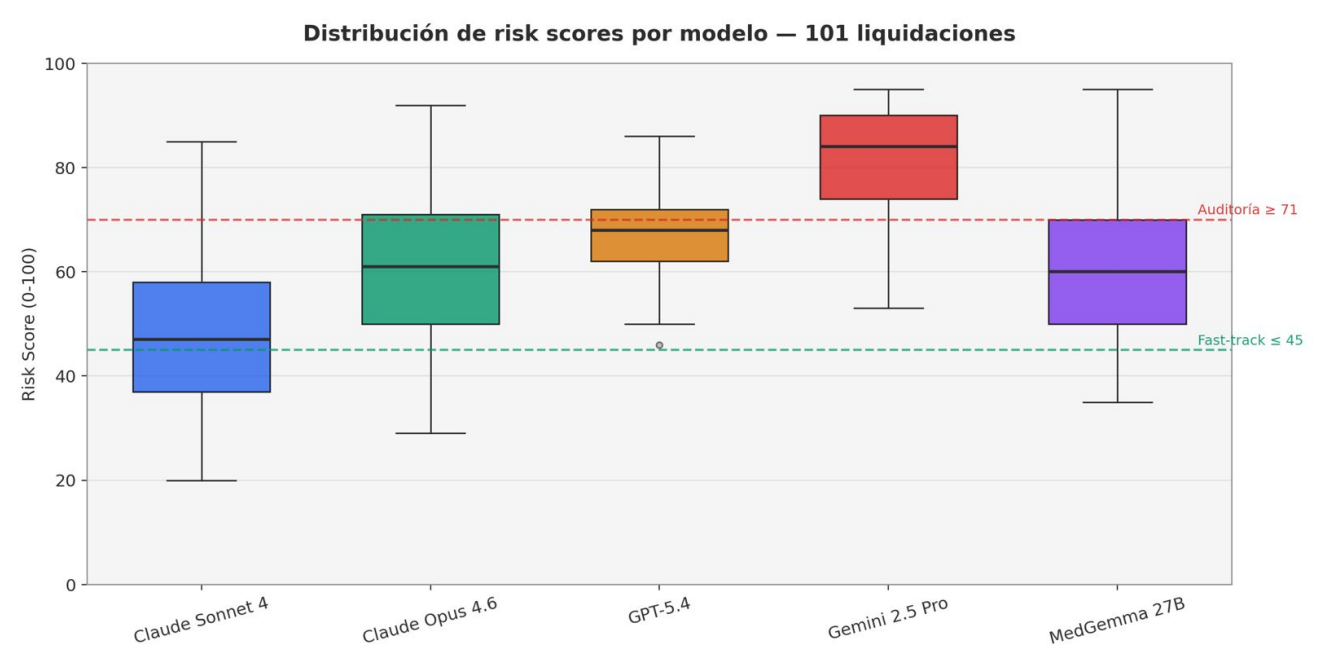
\includegraphics[width=0.96\textwidth,height=0.72\textheight,keepaspectratio]{images/p46_figure_1.png}
\caption{Distribución de puntajes de riesgo por modelo.}
\end{figure}

\textbf{GPT-5.4 resulta inviable para fast-track.} Con 0 \% de liquidaciones clasificadas como bajo riesgo, una desviación estándar de 8.8 y un puntaje mínimo de 42, GPT-5.4 trata todas las liquidaciones como si fueran de riesgo medio-alto. Su media de 69.3 está prácticamente en la frontera de auditoría completa. Un sistema que escala todo a revisión humana no aporta valor operativo. El hallazgo es relevante porque GPT-5.4 demostró buena profundidad clínica, lo que sugiere que su problema no es la falta de capacidad analítica sino un sesgo sistemático hacia la sobrepenalización.

Los tres modelos restantes resultaron inviables como modelo único, aunque por razones distintas. Opus genera el análisis más profundo del \textit{benchmark}, pero con solo 3.1 \% de fast-track y un costo 10x, funciona como segundo nivel, no como \textit{screening}. MedGemma, pese a su entrenamiento médico, obtuvo la menor profundidad y quedó limitado por su ventana de 8,192 \textit{tokens} y la necesidad de GPU dedicada. Gemini fue el más barato y el más confiable en \textit{parsing}, pero clasificó el 96 \% de los casos como de alto riesgo.

\begin{figure}[H]
\centering
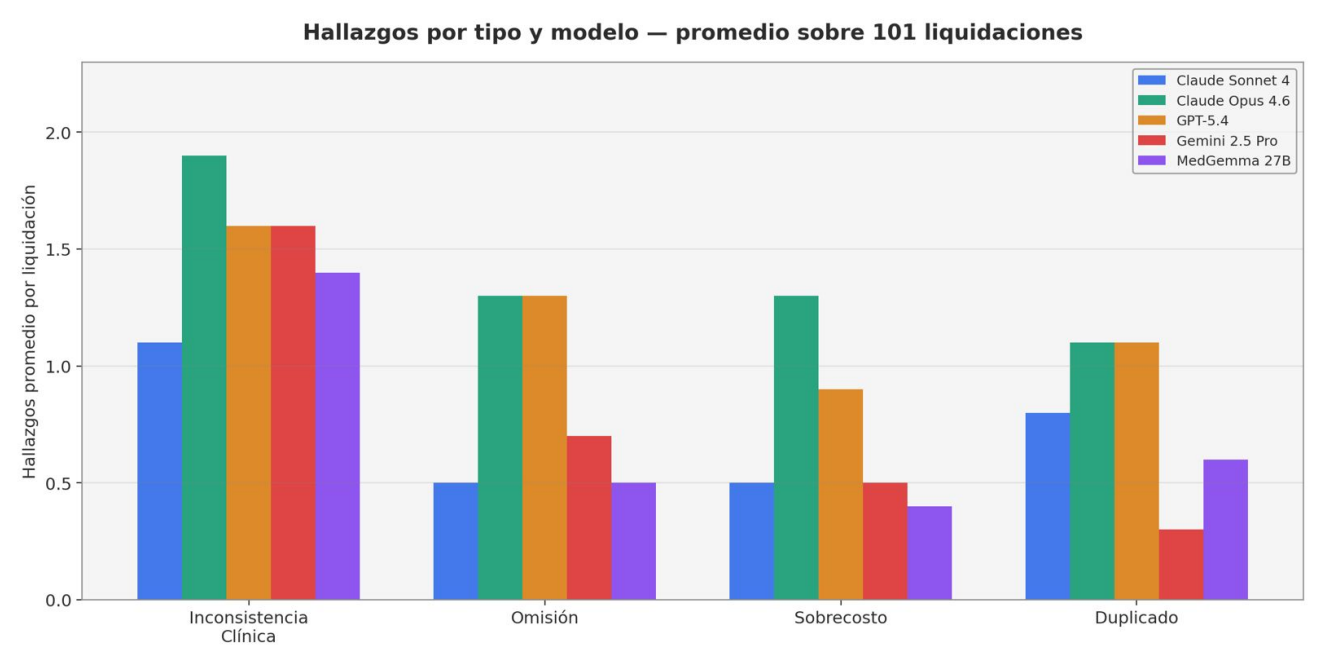
\includegraphics[width=0.96\textwidth,height=0.72\textheight,keepaspectratio]{images/p47_figure_1.png}
\caption{Promedio de hallazgos por liquidación, por tipo y modelo.}
\end{figure}

\textbf{Análisis de \textit{confounding}: ¿el volumen de ítems infla el puntaje?} Para cuantificar este efecto, se calculó la correlación entre el número total de ítems por liquidación y el \textit{risk score} asignado por cada modelo se presentan en la Tabla~\ref{tab:correlacion-items-risk-score}

\begin{table}[H]
    \centering
    \caption{Correlación entre número de ítems por liquidación y
    \textit{risk score}}
    \label{tab:correlacion-items-risk-score}

    \footnotesize
    \setlength{\tabcolsep}{7pt}
    \renewcommand{\arraystretch}{1.2}

    \begin{tabular}{
        l
        c
        c
        c
        c
        c
    }
        \toprule
        \textbf{Modelo}
        & \textbf{n}
        & \textbf{Pearson r}
        & \textbf{p-value}
        & \textbf{Spearman $\rho$}
        & \textbf{p-value} \\
        \midrule

        Claude Sonnet 4 & 101 & $-0.21$ & 0.035 & $-0.45$ & $< 0.001$ \\
        Claude Opus 4.6 & 98  & 0.04    & 0.732 & $-0.19$ & 0.064 \\
        GPT-5.4         & 99  & 0.03    & 0.808 & $-0.28$ & 0.004 \\
        Gemini 2.5 Pro  & 101 & $-0.07$ & 0.484 & $-0.28$ & 0.003 \\
        MedGemma 27B    & 101 & $-0.08$ & 0.427 & $-0.32$ & $< 0.001$ \\

        \bottomrule
    \end{tabular}
\end{table}

Ningún modelo muestra correlación positiva significativa entre volumen y \textit{score}. Sonnet, el modelo seleccionado para \textit{screening}, presenta una correlación negativa. Esto descarta la hipótesis de que la capacidad discriminativa de Sonnet sea un artefacto de la complejidad del caso. La discriminación por sigma es una condición necesaria, pero no suficiente: la validación de precisión a nivel de hallazgo requiere un piloto con auditor real.

\section{\textit{pipeline} integrado}

El \textit{pipeline} completo (Fase 1 + Fase 2 con estrategia escalonada, \textit{prompts} de producción e \textit{Identity Vault} activo) se ejecutó sobre las 101 liquidaciones del \textit{dataset} . A diferencia de las proyecciones de la sección 7.10, esta ejecución invocó el LLM real con la configuración de producción.

La distribución real de decisiones fue:

\begin{table}[H]
    \centering
    \caption{Distribución real de decisiones del \textit{pipeline} integrado}
    \label{tab:distribucion-decisiones-pipeline}

    \setlength{\tabcolsep}{10pt}
    \renewcommand{\arraystretch}{1.25}

    \begin{tabular}{
        l
        c
        c
        c
    }
        \toprule
        \textbf{Categoría}
        & \textbf{Cantidad}
        & \textbf{\% real}
        & \textbf{Proyección Sección~\ref{sec:resultados-preliminares}} \\
        \midrule

        \texttt{FAST\_TRACK}
        & 66
        & 65.3\,\%
        & 55--65\,\% \\

        \texttt{REVISION\_RAPIDA}
        & 9
        & 8.9\,\%
        & 15--20\,\% \\

        \texttt{AUDITORIA\_COMPLETA}
        & 26
        & 25.7\,\%
        & 10--15\,\% \\

        \texttt{RECHAZO\_ADMINISTRATIVO}
        & 0
        & 0.0\,\%
        & 3--5\,\% \\

        \bottomrule
    \end{tabular}
\end{table}

La tasa de recomendación de fast-track (65.3 \%) se ubica en el extremo superior del rango proyectado y casi triplica el 24.8 \% del \textit{benchmark} con Sonnet aislado. Esta tasa refleja la clasificación del \textit{pipeline}; la tasa efectiva de fast-track depende de la aceptación del auditor, un factor no medido en este alcance. La categoría AUDITORIA\_COMPLETA es mayor a lo proyectado porque el

LLM con \textit{prompts} de producción detecta inconsistencias clínicas que la simulación con puntajes fijos no capturaba. No hubo rechazos administrativos.

Los \textit{prompts} de producción y el pre-filtrado de Fase 1 produjeron un desplazamiento medible en la distribución de \textit{scores} de Sonnet en la tabla~\ref{tab:cambio-distribucion-scores-sonnet}:

\begin{table}[H]
    \centering
    \caption{Cambio en la distribución de \textit{scores} de Sonnet}
    \label{tab:cambio-distribucion-scores-sonnet}

    \footnotesize
    \setlength{\tabcolsep}{6pt}
    \renewcommand{\arraystretch}{1.25}

    \begin{tabular}{
        p{0.25\textwidth}
        p{0.25\textwidth}
        p{0.23\textwidth}
        p{0.13\textwidth}
    }
        \toprule
        \textbf{Métrica}
        & \textbf{\textit{Benchmark} (Sonnet aislado)}
        & \textbf{\textit{Pipeline} integrado}
        & \textbf{Cambio} \\
        \midrule

        Media del \textit{risk score}
        & 48.1
        & 38.6
        & $-9.5$ \\

        $\sigma$ del \textit{risk score}
        & 20.1
        & 24.9
        & $+4.8$ \\

        Mediana
        & ---
        & 25.0
        & --- \\

        Tasa de recomendación \textit{fast-track}
        & 24.8\,\% (umbral $\leq 30$)
        & 65.3\,\% (umbral $\leq 45$)
        & $+40.5$ pp \\

        Errores de \textit{parsing}
        & ---
        & 0 (Sonnet) / 0 (Opus)
        & --- \\

        \bottomrule
    \end{tabular}

    \vspace{2mm}

    \begin{minipage}{0.94\textwidth}
        \footnotesize
        \textit{Nota:} Los umbrales difieren entre ambas configuraciones
        ($\leq 30$ frente a $\leq 45$). La descomposición de factores se
        presenta en la tabla~\ref{tab:estudio-ablacion}
    \end{minipage}
\end{table}

Nota: Los umbrales difieren entre ambas configuraciones ($\leq$ 30 vs. $\leq$ 45). La descomposición de factores se presenta más adelante en la tabla~\ref{tab:estudio-ablacion}

De los 101 \textit{claims}, 33 (32.7 \%) fueron escalados a Opus. Los motivos de escalación, que pueden coexistir en un mismo \textit{claim}, fueron: \textit{score} Sonnet > 45 (26 \textit{claims}), hallazgo de alta severidad por inconsistencia clínica (14 \textit{claims}), y costo total > S/5,000 con ítems en revisión (9 \textit{claims}). Opus procesó los 33 \textit{claims} sin errores de \textit{parsing}, con un tiempo promedio de 25.2 segundos por caso.

\begin{figure}[H]
\centering
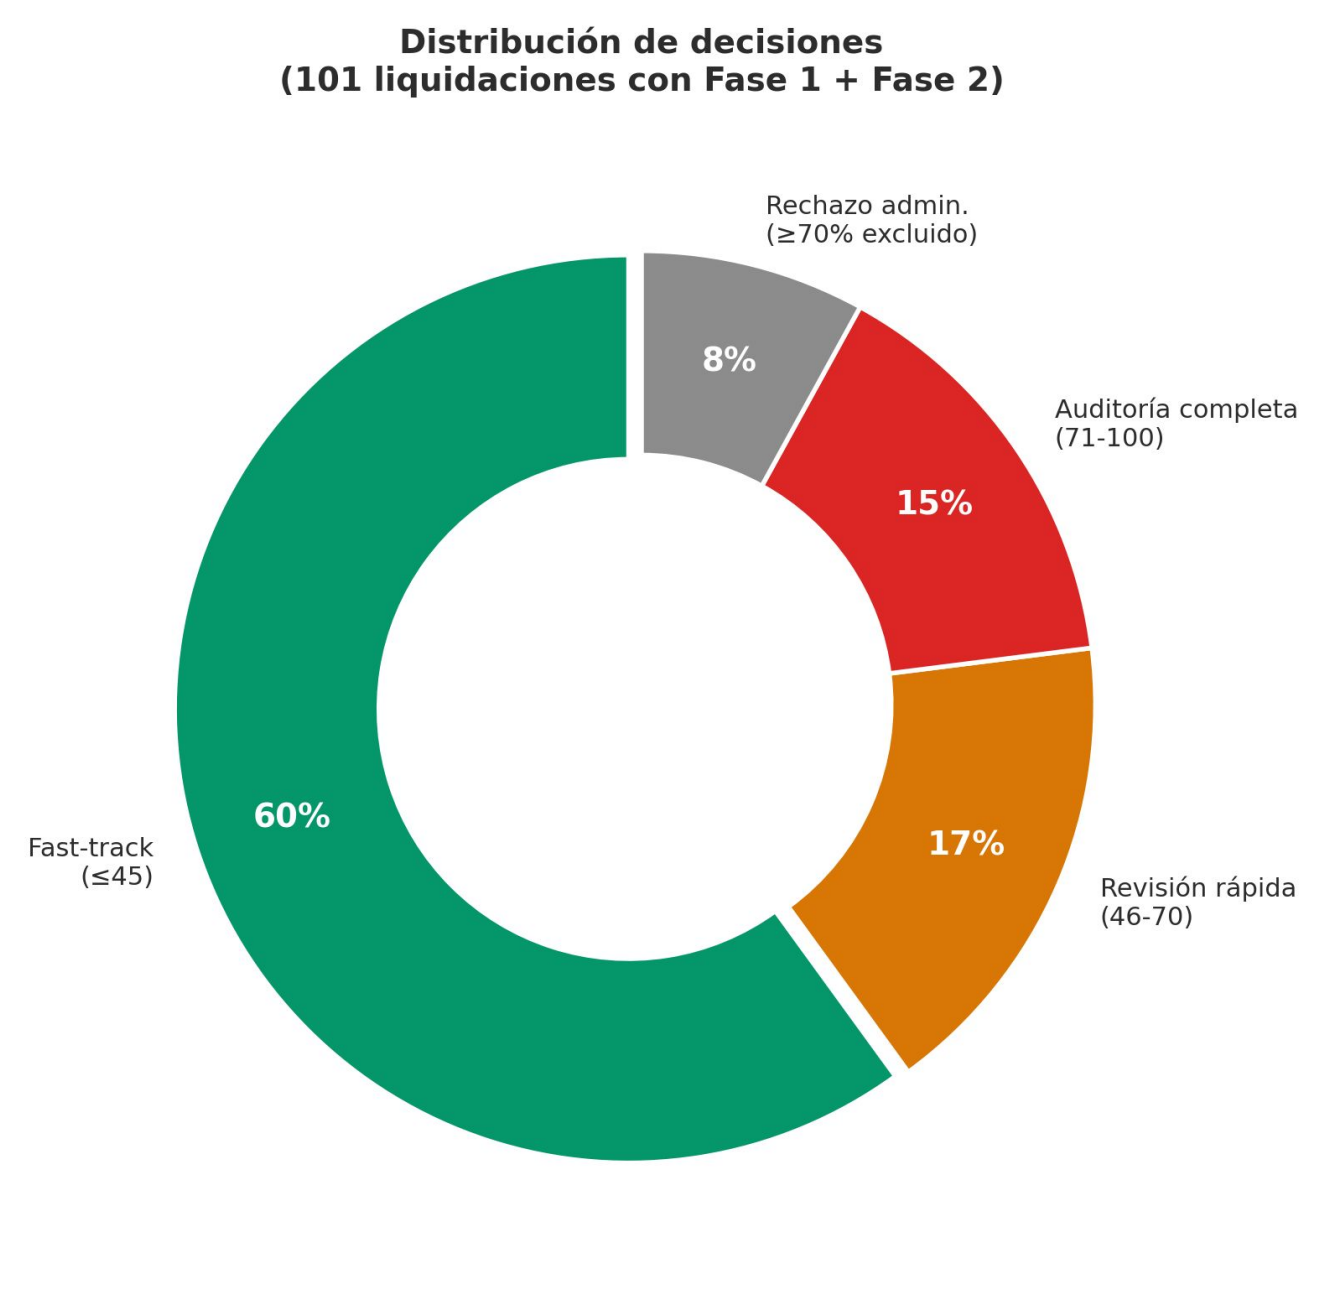
\includegraphics[width=0.96\textwidth,height=0.72\textheight,keepaspectratio]{images/p50_figure_1.png}
\caption{Distribución real de decisiones del \textit{pipeline} integrado.}
\label{p50_figure_1}
\end{figure}

\textbf{Nota sobre la comparación de umbrales.} La tasa de fast-track del \textit{benchmark} (24.8 \%) utilizó un umbral de $\leq$ 30, mientras que el \textit{pipeline} de producción emplea $\leq$ 45. Esta diferencia es el factor dominante en la mejora observada. Un estudio de ablación permite descomponer la contribución de cada factor:

\begin{table}[H]
    \centering
    \caption{Estudio de ablación de la mejora en la tasa de \textit{fast-track}}
    \label{tab:estudio-ablacion}

    \footnotesize
    \setlength{\tabcolsep}{6pt}
    \renewcommand{\arraystretch}{1.25}

    \begin{tabular}{
        p{0.27\textwidth}
        c
        p{0.16\textwidth}
        c
        c
        c
    }
        \toprule
        \textbf{Configuración}
        & \textbf{Umbral}
        & \textbf{\textit{Prompts}}
        & \textbf{Fase 1}
        & \textbf{Media del \textit{score}}
        & \textbf{\textit{Fast-track}} \\
        \midrule

        \textit{Benchmark} original
        & $\leq 30$
        & \textit{Benchmark}
        & No
        & 48.1
        & 24.8\,\% \\

        Solo cambio de umbral
        & $\leq 45$
        & \textit{Benchmark}
        & No
        & 48.1
        & 66.3\,\% \\

        \textit{Prompts} de producción, sin Fase 1
        & $\leq 45$
        & Producción
        & No
        & 37.9
        & 72.3\,\% \\

        \textit{Pipeline} completo
        & $\leq 45$
        & Producción
        & Sí
        & 38.6
        & 65.3\,\% \\

        \bottomrule
    \end{tabular}
\end{table}

El estudio de ablación descompone la mejora en tres efectos independientes:

\noindent \textbf{1. Cambio de umbral:} +41.6 pp.

\noindent \textbf{2. \textit{Prompts} de producción:} +6.0 pp.

\noindent \textbf{3. Fase 1 (pre-filtrado contractual):} -7.0 pp.

El valor de Fase 1 no está en aumentar la tasa de fast-track, sino en mejorar la calidad de la discriminación. Los \textit{claims} clasificados como fast-track con el \textit{pipeline} completo tienen mayor consistencia clínica verificada que los que habrían calificado solo con \textit{prompts} de producción.

El costo total de API fue de \$12.00 (\$2.83 para las 101 llamadas a Sonnet + \$9.17 para las 33 llamadas a Opus), con un tiempo total de ejecución de 38.9 minutos. El costo por \textit{claim} promedio fue de \$0.12.

Aplicando los tiempos estimados de revisión del auditor (1 min para fast-track, 10 min para revisión rápida, 45 min para auditoría completa), el tiempo total proyectado del lote sería de aproximadamente 21 horas, frente a las 75.8 horas del proceso manual, una reducción del 72 \%.

\section{Hallazgos clínicos de alto impacto}

Más allá de las métricas de distribución, el valor operativo del sistema se ilustra con los hallazgos que la Fase 2 señaló como candidatos a investigación durante el \textit{benchmark}. En cinco expedientes, el LLM identificó patrones de facturación que ameritan revisión por un auditor, por un monto acumulado superior a S/70,000. Ninguno de estos hallazgos constituye una determinación de fraude o de error, pero sí demuestran la capacidad del sistema para priorizar los casos que merecen atención humana.

Dos casos ilustran los patrones que el sistema escala para revisión humana. En una angioplastia valorada en aproximadamente S/39,460, los stents coronarios aparecen registrados como devueltos en el sistema de farmacia, pero el honorario por el procedimiento de implantación se mantuvo facturado. Un patrón similar se observó en una cirugía de fémur valorada en aproximadamente S/31,177, en la que la prótesis fue revertida, pero el cobro del procedimiento persistió. La inconsistencia entre la reversión del insumo de alto costo y el mantenimiento del honorario quirúrgico puede tener explicaciones operativas legítimas, pero también es consistente con patrones conocidos de facturación de procedimientos no completados.

En el ámbito de inconsistencias clínicas, el sistema detectó un expediente de un paciente geriátrico hospitalizado por neumonía donde se facturaron cero antibióticos, cero imágenes diagnósticas y cero broncodilatadores, una omisión farmacológica incompatible con el diagnóstico. En otro caso, alertó sobre la ausencia de profilaxis antitrombótica en una cirugía abdominal de una paciente de 83 años, una omisión que constituye un riesgo clínico grave según protocolos estándar.

Estos hallazgos ilustran que la Fase 2 aporta un valor que excede la verificación contractual de la Fase 1: la capacidad de cruzar el diagnóstico, los servicios facturados y los protocolos médicos esperados para señalar discrepancias que ameritan revisión humana.

\section{Validación con \textit{Golden Set}}

El \textit{Golden Set} de 17 liquidaciones, cuyas clasificaciones esperadas fueron validadas por un auditor médico externo al equipo, constituye el mecanismo de regresión y calibración del \textit{pipeline}. No es un conjunto de validación independiente, pero cumple una función operativa esencial: detectar degradaciones ante cambios en el sistema.

\textbf{Nivel 1: \textit{Routing} de Fase 1} Los 17 \textit{tests} parametrizados de test\_routing\_matches\_expected verifican que cada liquidación del \textit{Golden Set} recibe el \textit{routing} correcto. Los \textit{tests} de elegibilidad y cobertura también pasan.

\textbf{Nivel 2: Motor de decisión} Seis \textit{tests} simulan puntajes de Fase 2 para verificar que el motor de decisión produce las categorías esperadas. Se confirma, entre otros puntos, que el umbral de 45 es inclusivo y que la edad avanzada no genera una penalización automática.

\textbf{Nivel 3: Proyección de tasa} test\_projected\_rate\_meets\_target ejecuta Fase 1 sobre las 101 liquidaciones completas, simula Fase 2 y verifica que la tasa de fast-track se encuentra entre 55 \% y 75 \%.

\textbf{Diagnóstico de concordancia} La ejecución real del \textit{pipeline} logró una concordancia de 10/17 (58.8 \%) con las clasificaciones esperadas del \textit{Golden Set}. Esta cifra no constituye una métrica de rendimiento generalizable; su valor es diagnóstico. Revela que la tasa de falsos negativos fue del 0 \% y que los 7 \textit{mismatches} corresponden exclusivamente a sobre-escalaciones donde el LLM detectó inconsistencias clínicas que no eran evidentes en la revisión inicial del auditor.

\textbf{Estabilidad de umbrales \textit{(Leave-One-Out)}} Para evaluar si los umbrales dependen de algún caso individual del \textit{Golden Set}, se implementó un análisis \textit{leave-one-out}. Los 17 \textit{claims} pasan las verificaciones, confirmando que ningún caso individual es pivotal para la determinación del umbral.

\section{Análisis de costos}

El análisis económico compara tres estrategias de procesamiento con el costo manual tabla~\ref{tab:comparacion-estrategias-procesamiento}:

\begin{table}[H]
    \centering
    \caption{Comparación de estrategias de procesamiento}
    \label{tab:comparacion-estrategias-procesamiento}

    \footnotesize
    \setlength{\tabcolsep}{6pt}
    \renewcommand{\arraystretch}{1.3}

    \begin{tabular}{
        p{0.28\textwidth}
        p{0.23\textwidth}
        p{0.16\textwidth}
        p{0.25\textwidth}
    }
        \toprule
        \textbf{Estrategia}
        & \textbf{Costo por lote (101 \textit{claims})}
        & \textbf{Tiempo de API}
        & \textbf{Observación} \\
        \midrule

        Claude Sonnet 4 exclusivo
        & USD 2.83
        & $\sim 27.8$ min
        & Triaje eficiente, con menor profundidad clínica. \\

        Claude Opus 4.6 exclusivo
        & USD 28.08
        & $\sim 84.5$ min
        & Máxima profundidad, con un costo aproximadamente 10 veces mayor. \\

        Estrategia escalonada (Sonnet + Opus)
        & USD 12.00
        & $\sim 38.9$ min
        & Balance entre costo y calidad. \\

        Auditoría manual
        & 75.8 h $\times$ costo del auditor
        & 75.8 h
        & Línea base actual. \\

        \bottomrule
    \end{tabular}
\end{table}


El costo de la estrategia escalonada (\$12.00 por lote) representa menos del 0.001 \% del valor promedio de un lote hospitalario. El costo de API no es el factor limitante para la viabilidad económica del sistema; lo son la adopción por parte del auditor y la integración con los sistemas existentes.

\section{Cumplimiento de objetivos}

La siguiente tabla~\ref{tab:cumplimiento-objetivos} cruza cada objetivo específico con los resultados obtenidos:

\begin{table}[H]
    \centering
    \caption{Cumplimiento de los objetivos del proyecto}
    \label{tab:cumplimiento-objetivos}

    \footnotesize
    \setlength{\tabcolsep}{6pt}
    \renewcommand{\arraystretch}{1.3}

    \begin{tabular}{
        p{0.26\textwidth}
        p{0.19\textwidth}
        p{0.33\textwidth}
        p{0.16\textwidth}
    }
        \toprule
        \textbf{Objetivo}
        & \textbf{Meta}
        & \textbf{Resultado}
        & \textbf{Estado} \\
        \midrule

        OE1: Tasa de recomendación de \textit{fast-track}
        & 50--60\,\%
        & 65.3\,\% (66/101)
        & Cumplido \\

        OE2: Control de falsos positivos
        & Por definir en producción
        & No estimable con la evidencia disponible
        & No medido \\

        OE3: Tiempo por liquidación
        & $\leq 5$ min
        & $< 1$ min para \textit{fast-track};
          $\sim 17$ s de procesamiento del LLM
        & Cumplido \\

        Derivado: reducción del tiempo por lote
        & $\geq 40\,\%$
        & 57--72\,\%, según el escenario
        & Cumplido (estimado) \\

        Derivado: reducción del MLR
        & 1--2 puntos porcentuales
        & No medible sin un piloto real
        & No medido \\

        \bottomrule
    \end{tabular}
\end{table}

 \textbf{Sensibilidad de la reducción de tiempo.} La reducción de tiempo por lote depende de la confianza del auditor en el sistema. El siguiente (Tabla~\ref{tab:sensibilidad-reduccion-tiempo}) análisis muestra cómo varía bajo tres escenarios de adopción:

\begin{table}[H]
    \centering
    \caption{Sensibilidad de la reducción del tiempo por lote}
    \label{tab:sensibilidad-reduccion-tiempo}

    \footnotesize
    \setlength{\tabcolsep}{5pt}
    \renewcommand{\arraystretch}{1.25}

    \begin{tabular}{
        l
        c
        c
        c
        c
        c
    }
        \toprule
        \textbf{Escenario}
        & \textbf{t(\textit{fast-track})}
        & \textbf{t(rev. rápida)}
        & \textbf{t(aud. completa)}
        & \textbf{Total del lote}
        & \shortstack{\textbf{Reducción}\\\textbf{vs. 75.8 h}} \\
        \midrule

        Optimista
        & 1 min
        & 10 min
        & 45 min
        & 21.0 h
        & 72\,\% \\

        Conservador
        & 5 min
        & 15 min
        & 45 min
        & 27.2 h
        & 64\,\% \\

        Pesimista
        & 10 min
        & 20 min
        & 45 min
        & 32.5 h
        & 57\,\% \\

        \bottomrule
    \end{tabular}
\end{table}

Los tres escenarios superan la meta del 40 \%. Sin embargo, la reducción real depende de la confianza del auditor en el sistema, un factor que solo puede medirse en un piloto controlado.

 \textbf{Sensibilidad de la tasa efectiva de fast-track.} La tasa de recomendación de fast-track (65.3 \%) se convierte en tasa efectiva solo cuando el auditor acepta la recomendación:

\begin{table}[H]
    \centering
    \caption{Sensibilidad de la tasa efectiva de \textit{fast-track}}
    \label{tab:sensibilidad-fast-track-efectivo}

    \footnotesize
    \setlength{\tabcolsep}{7pt}
    \renewcommand{\arraystretch}{1.25}

    \begin{tabular}{
        p{0.32\textwidth}
        p{0.18\textwidth}
        p{0.16\textwidth}
        p{0.24\textwidth}
    }
        \toprule
        \textbf{Tasa de aceptación del auditor}
        & \textbf{\textit{Fast-track} efectivos}
        & \textbf{Tasa efectiva}
        & \textbf{Comparación con la meta de 50--60\,\%} \\
        \midrule

        90\,\%
        & 59
        & 58.8\,\%
        & Dentro de la meta \\

        80\,\%
        & 53
        & 52.2\,\%
        & Dentro de la meta \\

        70\,\%
        & 46
        & 45.7\,\%
        & Por debajo \\

        60\,\%
        & 40
        & 39.2\,\%
        & Por debajo \\

        \bottomrule
    \end{tabular}
\end{table}

Con una aceptación del 77 \% o superior, la tasa efectiva se mantiene dentro de la meta del 50 \%. Esta tasa de aceptación es plausible, pero solo puede confirmarse en un piloto con auditor real.

En síntesis, el MVP demuestra que la arquitectura funciona y que las proyecciones son favorables. Lo que no demuestra, porque no puede hacerlo dentro del alcance académico, es que el sistema produce los resultados esperados cuando un auditor real procesa un lote real con datos de producción. Esa validación requiere un piloto.

\addcontentsline{toc}{section}{CAPÍTULO XI}
\chapter{LIMITACIONES Y RIESGOS}

\section{Dataset}

El \textit{dataset}  de 101 liquidaciones tiene cuatro restricciones de generalización. Primera, proviene de un único plan de salud (MediVida). Las configuraciones de exclusiones, coberturas y medicamentos condicionales varían sustancialmente entre planes; el motor de Fase 1 requiere una configuración JSON por cada plan, y su precisión depende de la calidad de la extracción semiautomática desde el contrato PDF. Segunda, cubre exclusivamente liquidaciones hospitalarias. Las atenciones ambulatorias y odontológicas tienen estructuras de servicio, patrones de facturación e incentivos económicos distintos. Tercera, corresponde a un solo trimestre (Q3 2025), por lo que los patrones estacionales no están representados. Cuarta, el \textit{dataset}  no contiene casos confirmados de fraude, lo que impide evaluar la capacidad del sistema para detectar fraude, funcionalidad valorada por los \textit{stakeholders} pero excluida del alcance del MVP.

Quinta, el \textit{Golden Set} de 17 liquidaciones fue clasificado por un único auditor médico, sin medición de acuerdo inter-evaluador. Esto impide establecer un \textit{ceiling} de concordancia humana: la concordancia del 58.8 \% entre el pipeline y el auditor no puede interpretarse sin saber cuál sería la concordancia entre dos auditores humanos sobre los mismos 17 casos.

\section{Modelo}

El \textit{benchmark} documentó dos sesgos del LLM que afectan la calidad de las decisiones.

\textbf{Sobre-detección en reversiones y ajustes administrativos} Los modelos interpretan las reversiones en farmacia como señales de riesgo, cuando frecuentemente reflejan ajustes administrativos normales del sistema de dispensación de la IPRESS. En el caso H0710170, tanto Opus como Sonnet marcaron un patrón de 15 reversiones como hallazgo de riesgo medio, cuando en realidad representaban un cambio de presentación de medicamento registrado como reversión más nuevo cargo. Los \textit{prompts} anti-sesgo mitigan parcialmente este problema, pero no lo eliminan.

\textbf{Inflación por volumen} Opus y GPT-5.4 asignan puntajes más altos a liquidaciones con muchos ítems, incluso cuando la consistencia clínica es adecuada. La solución parcial es la instrucción explícita de no penalizar por volumen de ítems si son clínicamente consistentes. Sin embargo, el análisis de correlación mostrado en la sección 10.1 indica que este sesgo no afecta a Sonnet de forma sistemática: la correlación entre número de ítems y \textit{risk score} es negativa.

Opus presentó 3 errores de \textit{parsing} (3.0 \%) y GPT-5.4 presentó 2 (2.0 \%). En el pipeline de producción, un error de \textit{parsing} en Sonnet dispara la escalación a Opus; si Opus también falla, el caso se deriva a auditoría completa. Este mecanismo de \textit{fallback} evita que un error técnico produzca una decisión automatizada sobre un caso no evaluado, pero introduce latencia adicional y costo.

\textbf{Ausencia de \textit{test-retest}} El benchmark ejecutó cada par \textit{claim}-modelo una sola vez. Sin repeticiones, no es posible calcular la variabilidad intra-\textit{claim}. La desviación estándar reportada mide la variación entre \textit{claims}, no la estabilidad del \textit{score} para un mismo \textit{claim}. En producción, la temperatura 0.1 mitiga esta limitación al reducir la estocasticidad del modelo, pero no la elimina. Un benchmark con 3 a 5 repeticiones por \textit{claim} permitiría calcular intervalos de confianza y estimar la tasa de \textit{claims} en la zona de decisión inestable.

\section{Operativas}

La dependencia de APIs externas constituye el riesgo operativo principal. Tanto Sonnet como Opus se consumen vía la API de Anthropic \cite{anthropic2025claude}. Una interrupción del servicio bloquea la Fase 2 del \textit{pipeline}. El manejo de errores implementado en orchestrator.py contempla \textit{timeouts}, reintentos y \textit{fallback}, pero no elimina la dependencia. En un escenario de producción con miles de liquidaciones diarias, el SLA de la API de Anthropic se convierte en un componente crítico de la arquitectura.

La latencia acumulada también es una consideración. Sonnet toma alrededor de 17 segundos por caso; si se escala a Opus, se agregan cerca de 50 segundos adicionales. Para un lote de 101 liquidaciones procesadas secuencialmente, la Fase 2 toma entre 28 minutos y 70 minutos. Esto es aceptable para procesamiento por lotes, pero insuficiente para triaje en tiempo real si la aseguradora requiriese decisiones instantáneas.

\section{Adopción}

La barrera de adopción más significativa no es técnica sino organizacional. El auditor médico tiene una trayectoria profesional construida sobre su juicio clínico individual. Un sistema que clasifica como fast-track el 60 \% de los casos podría ser percibido como una amenaza a su relevancia profesional, no como una herramienta de productividad. La interfaz de NexusCare mitiga este riesgo de tres maneras: expone la justificación clínica completa junto a cada puntaje, preserva el \textit{override} humano obligatorio y separa los hallazgos por tipo y severidad para que el auditor pueda evaluar rápidamente si el sistema ha identificado algo que él habría pasado por alto.

La concordancia auditor-sistema, la métrica que valida la adopción, solo puede medirse en un piloto con usuarios reales. El MVP la registra en la interfaz pero no la ha medido.

\section{Regulatorios}

El marco normativo peruano presenta tanto protecciones como vacíos respecto a la automatización de decisiones en salud. La Ley No 29733 de Protección de Datos Personales \cite{peru2011ley29733} establece requisitos claros sobre el tratamiento de datos sensibles de salud, que \textbf{\textit{NexusCare}} aborda mediante el \textit{Identity Vault} y la anonimización previa al LLM. Sin embargo, la normativa de SUSALUD no contempla explícitamente el uso de inteligencia artificial en la adjudicación de liquidaciones médicas. No existe una prohibición, pero tampoco una autorización o marco regulatorio específico.

Esta ambigüedad implica que un despliegue en producción requeriría consulta previa con SU- SALUD y, probablemente, la implementación del sistema como herramienta de soporte, no de decisión, hasta que se desarrolle normativa específica. Esa es precisamente la posición que NexusCare adopta al mantener el \textit{human-in-the-loop} obligatorio.

El EU AI Act \cite{eu2024aiact} clasifica los sistemas de IA en salud como de alto riesgo, requiriendo supervisión humana, trazabilidad y evaluación de conformidad. De manera complementaria, la OMS establece que la ética y los derechos humanos deben ocupar un lugar central en el diseño, despliegue y uso de sistemas de inteligencia artificial para la salud, junto con mecanismos de gobernanza que aseguren la responsabilidad de los actores involucrados \cite{who2021ethics}. Aunque estos marcos no son vinculantes en el Perú, sirven como referencia normativa y anticipan la dirección regulatoria probable en la región. \textbf{\textit{NexusCare}} cumple con estos principios mediante supervisión humana, trazabilidad y evaluación de conformidad.

\addcontentsline{toc}{section}{CAPÍTULO XII}
\chapter{APRENDIZAJES Y LECCIONES}

\section{Técnicos}

Los modelos generalistas de frontera (\textit{Claude Sonnet}, \textit{Claude Opus}) superaron al modelo especialista médico (MedGemma 27B) en una tarea que, en principio, debería favorecer al especialista. MedGemma está entrenado con corpus médicos y entiende terminología clínica. Sin embargo, la tarea de auditoría de liquidaciones no es puramente médica: requiere razonamiento sobre datos tabulares heterogéneos (códigos, descripciones, costos), detección de patrones administrativos (reversiones, duplicados) y evaluación de proporcionalidad económica. Estas capacidades dependen más de la escala y la versatilidad del modelo que de su especialización en el dominio clínico. La ventana de contexto de 8,192 \textit{tokens} de MedGemma fue una limitación adicional que obligó a truncar la información de entrada, perdiendo visibilidad sobre los ítems de cola larga donde frecuentemente se esconden los sobrecostos.

Dos hallazgos operativos complementan esta lección. La desviación estándar, como métrica de discriminación, resultó ser el indicador más predictivo de utilidad: si el equipo hubiese seleccionado por media de puntaje o de número de hallazgos, habría elegido Opus, un modelo que discrimina poco y no genera clasificaciones \textit{fast-track}. Y el pre-filtrado de Fase 1 aportó un valor imprevisto pero contra-intuitivo: al inyectar el contexto de cobertura contractual en el \textit{prompt} del LLM, no redujo la tasa de sobre-escalación sino que la aumentó en 7 pp (de 72.3 \% a 65.3 \% de fast-track, según el estudio de ablación de §10.2). El valor de Fase 1 no está en reducir falsos positivos sino en mejorar la calidad de la discriminación: los 7 \textit{claims} adicionales que se escalan son precisamente aquellos con discrepancias contractuales que el LLM, sin contexto de cobertura, habría ignorado. La sinergia entre el motor de reglas y el LLM no es aditiva (ambos reducen riesgo) sino complementaria (cada uno detecta un tipo distinto de anomalía).

\section{Metodológicos}

El \textit{Golden Set} de 17 liquidaciones resultó más útil de lo esperado para un conjunto tan pequeño. Su función no es estadística (17 casos no prueban nada en sentido inferencial), sino de calibración y regresión. Lo que le da credibilidad es que las clasificaciones esperadas fueron definidas por un auditor médico, no por el equipo técnico: el \textit{Golden Set} refleja criterio clínico experto, no una expectativa autorreferencial. Cada vez que se modificó un umbral, se ajustó un \textit{prompt} o se cambió la lógica de \textit{routing}, el \textit{Golden Set} respondió a la pregunta operativa inmediata: “¿este cambio rompe algún caso que antes funcionaba?” Los 59 \textit{tests} del \textit{Golden Set}   (test golden set.py), 51 parametrizados sobre los 17 \textit{claims}, más 6 de simulación de decisión y 2 de proyección de tasa, se ejecutan en menos de 3 segundos y cubren \textit{routing}, elegibilidad, cobertura y la decisión final. Sin este mecanismo, la calibración de umbrales habría sido un proceso de ensayo y error sin retroalimentación inmediata.

La estrategia escalonada (Sonnet para \textit{screening}, Opus para análisis profundo) constituye un patrón reutilizable más allá de este proyecto. El principio subyacente (usar un modelo rápido y barato para filtrar, y uno lento y caro para profundizar) aplica a cualquier flujo de trabajo donde la distribución de complejidad sea asimétrica (muchos casos simples, pocos complejos). Los criterios de escalación (nexuscare/pipeline/escalation.py) encapsulan la lógica de forma parametrizable: umbrales de \textit{score}, tipos de hallazgo, costo total del caso. Esto permite ajustar la agresividad de la escalación según el contexto operativo sin modificar la arquitectura.

\section{De negocio}

La heterogeneidad de datos que se describe en la sección 2.3 como un problema teórico resultó ser una barrera práctica concreta durante el desarrollo. La extracción de reglas de plan desde los contratos PDF de MediVida consumió más tiempo del previsto porque los contratos utilizan lenguaje ambiguo (“se cubrirán los medicamentos indicados excepto los expresamente excluidos”), referencias cruzadas entre secciones y tablas con formatos inconsistentes. El proceso semiautomático (LLM extrae, humano valida) redujo el esfuerzo, pero cada nuevo plan requiere entre 4 y 8 horas de configuración y validación. En un escenario con decenas de planes activos, como operan las EPS grandes, esto implica un costo operativo recurrente que debe dimensionarse en el modelo de negocio.

La brecha entre la viabilidad técnica y la adopción operativa se hizo evidente durante las conversaciones informales con auditores. El sistema puede procesar 101 liquidaciones en menos de 2 horas; la pregunta operativa no es “¿funciona?” sino “¿quién firma la decisión de clasificar como fast-track ?” En el contexto regulatorio peruano, una liquidación clasificada como fast-track que resulte en una glosa de SUSALUD recae sobre la persona que autorizó la aprobación, no sobre el sistema. Hasta que la normativa se adapte al uso de IA como herramienta de soporte, o hasta que la experiencia acumulada genere confianza institucional, la fast-track operará como una pre-aprobación que el auditor ratifica con un clic, no como una decisión final sin intervención humana.

\addcontentsline{toc}{section}{CAPÍTULO XIII}
\chapter{CONCLUSIONES}

\section{Validación Preliminar del MVP}

La hipótesis de valor del MVP, que un sistema de dos fases (reglas contractuales + LLM) puede clasificar las liquidaciones hospitalarias con suficiente precisión para reducir el tiempo de auditoría en un 40 \%, recibió evidencia favorable pero no fue validada en producción. La arquitectura es viable (0 errores de ejecución, 0 errores de \textit{parsing} en 101 liquidaciones),

La tasa de recomendación de \textit{fast-track} alcanzó el 65.3 \%, por encima del rango meta de 50– 60 \%. Una tasa más alta de la esperada podría indicar que el umbral de decisión es demasiado permisivo y que se están dejando pasar casos que merecerían revisión. Dicho esto, hay dos razones para no alarmarse todavía. Por un lado, el resultado está lejos del techo de alerta del 75 \% que definimos en §9.3 como señal de calibración insuficiente. Por otro, ninguno de los 17 casos del \textit{Golden Set} que debían escalarse fue clasificado erróneamente como fast-track, es decir, la tasa de falsos negativos observada es cero. El problema es que 17 casos son pocos para hacer una afirmación fuerte al respecto, y además esos mismos casos se usaron para calibrar los umbrales, con lo cual hay un sesgo inherente. En la práctica, la pregunta de si el 65.3 \% es seguro o riesgoso solo puede responderla un piloto con auditores reales procesando lotes de producción. Lo que sí podemos afirmar es que el exceso sobre la meta se explica principalmente por la recalibración de umbrales y, en menor medida, por los \textit{prompts} anti-sesgo, como muestra el estudio de ablación de §10.2. Si en el piloto la tasa de falsos negativos supera el 2 \%, la acción inmediata sería bajar el umbral de 45 a un valor más conservador.

El análisis de sensibilidad muestra que la reducción de tiempo supera el 40 \% incluso en el escenario más pesimista (57 \%). Sin embargo, la reducción de tiempo depende de supuestos sobre el comportamiento del auditor que no han sido medidos, y la concordancia del \textit{Golden Set} (58.8 \%) revela una tasa de sobre-escalación que requiere calibración adicional. La validación operativa con un auditor real en producción queda pendiente; el MVP deja preparada la infraestructura para ello.

Los datos que sustentan esta afirmación son tres. Primero, el \textit{benchmark} de 505 evaluaciones demostró que Claude Sonnet 4 discrimina entre casos de bajo y alto riesgo con una distribución equilibrada ($\sigma$ = 20.1), lo que habilita la clasificación automática. Segundo, el \textit{pipeline} integrado (Fase 1 + Fase 2 con estrategia escalonada) procesó las 101 liquidaciones sin errores, produciendo 66 fast-track (65.3 \%), 9 revisiones rápidas (8.9 \%) y 26 auditorías completas (25.7 \%), con un costo total de API de USD 12.00 en 38.9 minutos. Tercero, el \textit{Golden Set} de 17 casos, diseñado como herramienta de regresión y calibración y no como conjunto de validación independiente, mostró una concordancia de 10/17 (58.8 \%) con el \textit{pipeline} real. Los 7 \textit{mismatches} son sobre-escalaciones (falsos positivos, no falsos negativos), lo que indica una dirección segura del error pero también un margen de calibración pendiente.

Lo que falta es la validación con el usuario final. La métrica de concordancia auditor-sistema y la tasa de falsos positivos en condiciones reales solo pueden obtenerse mediante un piloto controlado. El MVP deja preparada la infraestructura para esa medición (interfaz con registro de acciones, \textit{logging} de \textit{pipeline}), pero el dato no existe aún.

\section{Contribución}

\textbf{\textit{NexusCare}} aporta dos elementos concretos al estado del arte de la auditoría médica automatizada en el Perú. Lo más transferible es la demostración de que la arquitectura de dos fases (reglas + LLM) complementa al LLM único en una dimensión que el LLM solo no cubre: la verificación contractual determinística. El estudio de ablación (§10.2) mostró que Fase 1 no mejora la tasa de fast-track (el LLM con \textit{prompts} calibrados alcanza un 72.3 \% sin contexto contractual), pero sí mejora la calidad de la discriminación al escalar los 7 \textit{claims} con discrepancias contractuales que el LLM ignoraba. En dominios donde conviven reglas de negocio explícitas con juicios que requieren razonamiento sobre lenguaje natural, la combinación no es aditiva sino complementaria: las verificaciones contractuales son determinísticas y reproducibles, mientras que el LLM se concentra en lo que genuinamente aporta, el razonamiento clínico contextual. El segundo es el benchmark comparativo de cinco modelos sobre datos reales del sector salud peruano: la superioridad del generalista sobre el especialista, la importancia de sigma como métrica de discriminación y la inviabilidad de GPT-5.4 por sobre-penalización son hallazgos empíricos reproducibles. No se encontró literatura previa que compare modelos de lenguaje en esta tarea específica, ni en el Perú ni en la región.

El diseño del \textit{pipeline} con \textit{privacy by design}, trazabilidad y \textit{Golden Set} para regresión continua complementa la contribución, aunque responde más a buenas prácticas de ingeniería que a una innovación metodológica.

\section{Viabilidad}

La viabilidad técnica está demostrada: el \textit{pipeline} procesa 101 liquidaciones sin errores fatales, los 190 \textit{tests} pasan, el costo de API es marginal frente al valor de las liquidaciones, y la latencia es compatible con procesamiento por lotes.

La viabilidad económica es favorable con reservas. El costo de API medido (USD 12.00 por lote con estrategia escalonada, 33 \% de escalación a Opus) es insignificante. El ahorro operativo estimado (de 75.8 horas a 21–32.5 horas según el escenario de adopción, una reducción del 57–72 \%) justifica la inversión en desarrollo y mantenimiento del sistema. La reserva es la dependencia del \textit{pricing} de Anthropic: un aumento significativo en los precios de API alteraría la ecuación, aunque el sistema soporta la migración a otros modelos (Gemini, por ejemplo, a USD 1.78 por lote).

La viabilidad operativa es la más incierta. Requiere tres condiciones que no dependen del equipo técnico: (a) disposición de una EPS/IAFAS a participar en un piloto con datos de producción, (b) aceptación del auditor médico del flujo de trabajo propuesto, y (c) claridad regulatoria de SUSALUD sobre el uso de IA como herramienta de soporte en la adjudicación de liquidaciones. Sin estas tres condiciones, \textbf{\textit{NexusCare}} permanece como un proyecto académico técnicamente validado.

\addcontentsline{toc}{section}{CAPÍTULO XIV}
\chapter{TRABAJO FUTURO}

\section{Corto plazo (3–6 meses)}

La prioridad inmediata es un piloto controlado con una IAFAS. El piloto requeriría: acceso a las liquidaciones de producción (no las 101 del \textit{dataset}  actual, sino lotes operativos con diversidad de planes y tipos de atención), la participación de al menos dos auditores médicos para medir la concordancia y los falsos positivos, y un periodo mínimo de 3 meses para capturar la variabilidad temporal. El diseño experimental debería incluir un grupo de control (auditoría manual) y un grupo de tratamiento (auditoría asistida por \textbf{\textit{NexusCare}}), y medir el tiempo total de cierre del lote como variable principal.

Un \textit{feature} crítico pendiente es la verificación de precios: comparar los montos liquidados por la IPRESS con los precios efectivamente convenidos con la IAFAS. Para medicamentos, las fuentes de referencia son el Observatorio Privado de Precios de Medicamentos (OPPM) de APEPS, que reporta precios reales del mercado de boticas, y Kairos, que publica precios de lista de laboratorios. La integración de estas fuentes permitiría detectar automáticamente sobrecostos en la Capa 1 del \textit{pipeline}, antes de que el caso llegue al análisis clínico.

En paralelo, la configuración del sistema debe ampliarse a más planes de salud. El proceso de extracción de reglas desde PDF contractuales (nexuscare/plan extraction/) ya está implementado, pero cada plan requiere validación humana. La prioridad sería configurar los 3–5 planes con mayor volumen de liquidaciones de la EPS piloto.

La calibración de umbrales debe incorporar el \textit{feedback} del auditor. El \textit{Golden Set} actual de 17 casos es un punto de partida; con datos de producción, puede expandirse a 50–100 casos con clasificaciones confirmadas por el auditor, lo que permitiría una calibración con mayor representatividad estadística.

\section{Mediano plazo (6–18 meses)}

La extensión a liquidaciones ambulatorias y odontológicas duplicaría el mercado direccionable del sistema. Las atenciones ambulatorias operan bajo CPM (no FFS), lo que cambia los incentivos de facturación y los tipos de inconsistencia relevantes. El motor de Fase 1 requeriría nuevas configuraciones de reglas, y los \textit{prompts} de Fase 2 necesitarían adaptarse a las diferencias clínicas (las ambulatorias son más breves, con menos ítems pero mayor volumen).

La integración con TEDEF y los ERPs de las IPRESS eliminaría la etapa de ingesta manual. En la actualidad, las liquidaciones se reciben como archivos JSON pre-normalizados. Una integración directa con TEDEF permitiría el procesamiento automatizado de lotes a medida que se reciben, reduciendo el ciclo de cierre. La complejidad principal no es técnica sino organizacional: TEDEF opera bajo estándares definidos por SUSALUD, y cualquier integración requiere certificación.

Un módulo de detección de fraude podría complementar la auditoría de consistencia clínica. Los patrones de fraude más comunes en el sector (procedimientos fantasma, facturación duplicada de dispositivos de alto valor, \textit{upcoding}) requieren análisis longitudinales (comparación entre liquidaciones del mismo prestador) que exceden el alcance del análisis caso por caso actual. Este módulo necesitaría acceso a datos históricos agregados, lo que plantea desafíos adicionales de privacidad y almacenamiento.

\section{Largo plazo}

La evolución natural del sistema apunta a un modelo SaaS \textit{multi-tenant} para múltiples EPS/IAFAS, con la adopción de FHIR como formato nativo, lo que facilita una eventual expansión regional. Colombia, Chile y México enfrentan problemas de auditoría similares con marcos regulatorios en evolución. Como línea de investigación, el hallazgo de que el modelo generalista supera al especialista en esta tarea merece validación en otros dominios clínicos donde el conocimiento especializado podría ser más determinante, como radiología, patología y genómica.





%% ============================================================================
\renewcommand{\bibname}{\centering\Large\bf{REFERENCIAS BIBLIOGR\'AFICAS}}
\addcontentsline{toc}{section}{REFERENCIAS BIBLIOGRÁFICAS}
\bibliographystyle{IEEEtran} 
\bibliography{referencias}   % The references are in "referencias.bib"

\anexossection
\addcontentsline{toc}{section}{ANEXOS} 
\markboth{ANEXOS}
\begin{Glosario}
    \centering
    \caption{Glosario de términos}
    \label{tab:glosario-terminos}

    \footnotesize
    \setlength{\tabcolsep}{6pt}
    \renewcommand{\arraystretch}{1.25}

    \begin{tabular}{
        p{0.20\textwidth}
        p{0.72\textwidth}
    }
        \toprule
        \textbf{Término}
        & \textbf{Definición} \\
        \midrule

        CIE-10 (ICD-10)
        & Clasificación Internacional de Enfermedades, décima revisión.
          Estándar de la OMS para codificación de diagnósticos médicos. \\

        CPT
        & \textit{Current Procedural Terminology}. Sistema de codificación
          de procedimientos médicos de la AMA. \\

        EPS
        & Entidad Prestadora de Salud. Organización que administra planes
          de salud complementarios en el Perú. \\

        FHIR
        & \textit{Fast Healthcare Interoperability Resources}. Estándar de
          interoperabilidad de datos clínicos de HL7 International. \\

        \textit{Golden Set}
        & Conjunto curado de liquidaciones con clasificaciones esperadas,
          utilizado para regresión y calibración. \\

        IAFAS
        & Institución Administradora de Fondos de Aseguramiento en Salud.
          Entidad que administra fondos de seguro de salud. \\

        IPRESS
        & Institución Prestadora de Servicios de Salud. Clínica u hospital
          que brinda atención y presenta liquidaciones. \\

        LLM
        & \textit{Large Language Model}. Modelo de lenguaje de gran escala
          entrenado sobre corpus textuales masivos. \\

        MLR
        & \textit{Medical Loss Ratio}. Razón entre siniestros pagados y primas
          cobradas; indicador de eficiencia de la aseguradora. \\

        MVP
        & \textit{Minimum Viable Product}. Versión mínima funcional del producto
          que permite validar hipótesis de negocio. \\

        PII
        & \textit{Personally Identifiable Information}. Datos que permiten
          identificar a una persona natural. \\

        SUSALUD
        & Superintendencia Nacional de Salud. Ente regulador del sistema
          de salud en el Perú. \\

        TEDEF
        & Plataforma de intercambio electrónico de datos entre EPS e IPRESS
          para liquidaciones y acreditación. \\

        \bottomrule
    \end{tabular}
\end{table}


    

\end{document}
%% ----------------------------------------------------------------
